\addtocontents{toc}{\setcounter{tocdepth}{-10}}

\chapter{Appendices}

\section{Initial Project Idea}\label{appendix:initIdea}
\begin{figure}[!htbp]
    \centering
    \noindent\begin{subfigure}[b]{\textwidth}
        \centering
        \frame{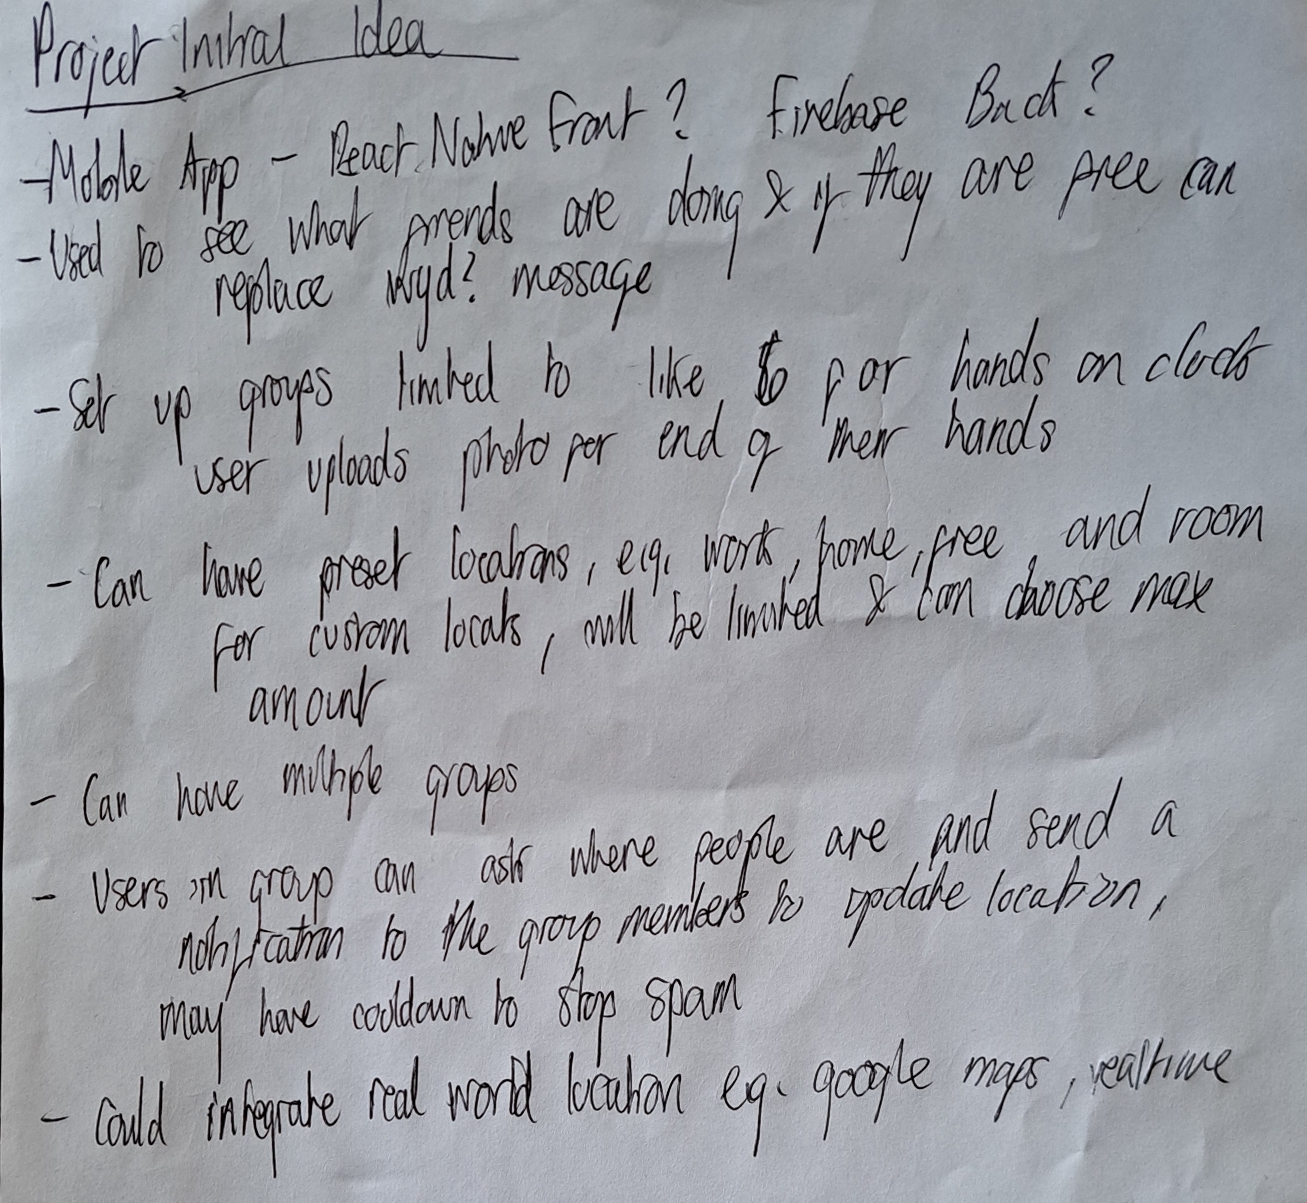
\includegraphics[width=\textwidth]{initialProjectIdea.jpg}}
    \end{subfigure}
\caption{Initial Project Idea}
\end{figure}
\FloatBarrier
\newpage


\section{Figma Designs}\label{appendix:figmaScreens}
\begin{figure}[!htbp]
    \centering
    \noindent\begin{subfigure}[b]{0.23\textwidth}
        \centering
        \frame{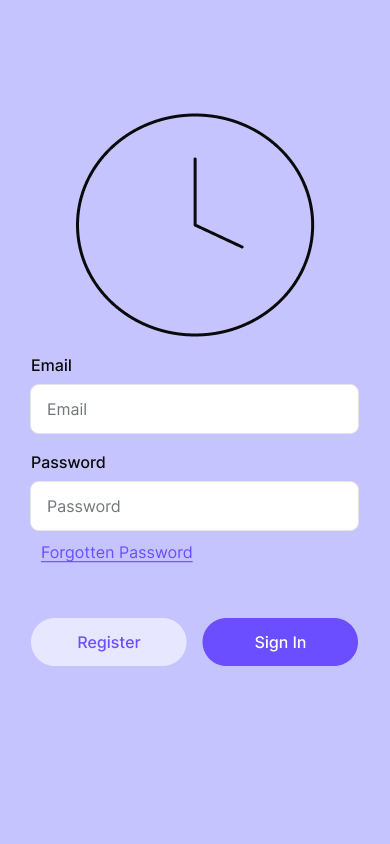
\includegraphics[width=\textwidth]{designSignIN.png}}
        \caption{Sign In}
    \end{subfigure}
    \hspace{0.5em}
    \noindent\begin{subfigure}[b]{0.23\textwidth}
        \centering
        \frame{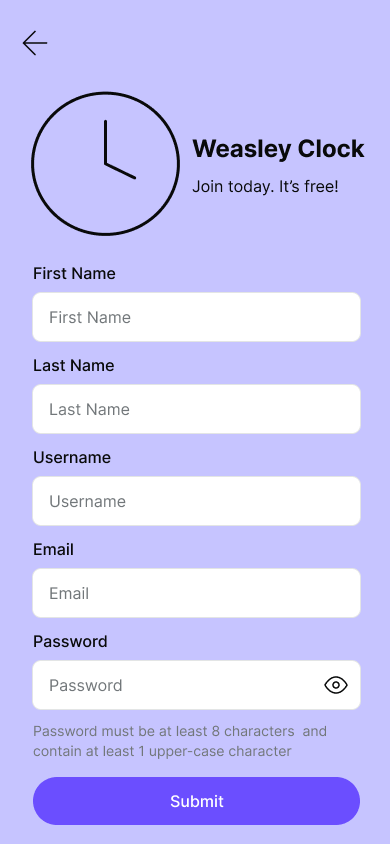
\includegraphics[width=\textwidth]{designRegister.png}}
        \caption{Register}
    \end{subfigure}
    \hspace{0.5em}
    \noindent\begin{subfigure}[b]{0.23\textwidth}
        \centering
        \frame{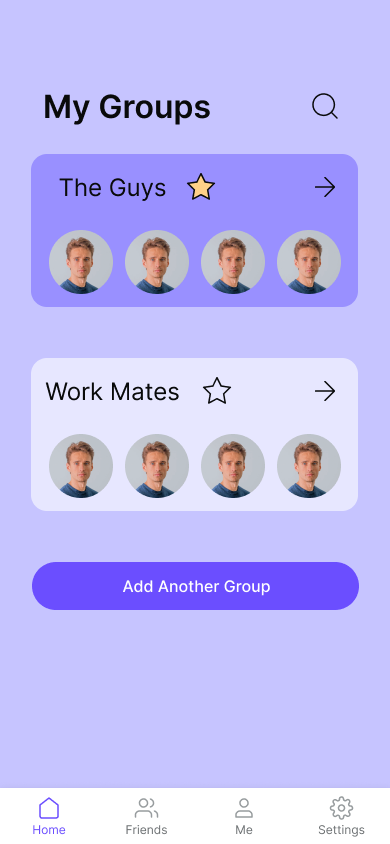
\includegraphics[width=\textwidth]{designHome.png}}
        \caption{Home}
    \end{subfigure}
    \hspace{0.5em}
    \noindent\begin{subfigure}[b]{0.23\textwidth}
        \centering
        \frame{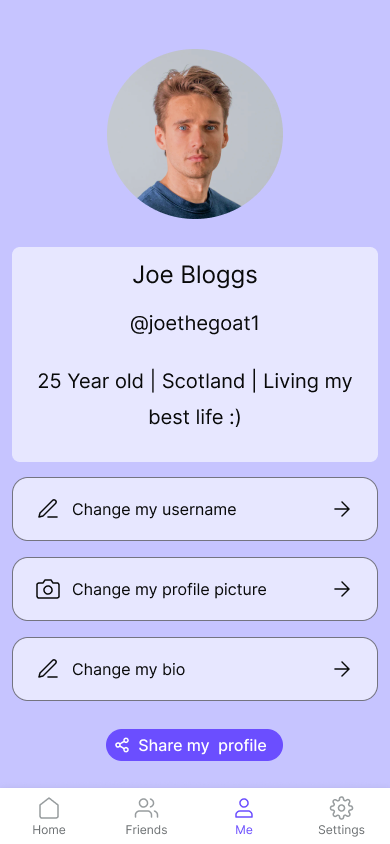
\includegraphics[width=\textwidth]{designProfile.png}}
        \caption{User Profile}
    \end{subfigure}
    \vskip\baselineskip
    \noindent\begin{subfigure}[b]{0.23\textwidth}
        \centering
        \frame{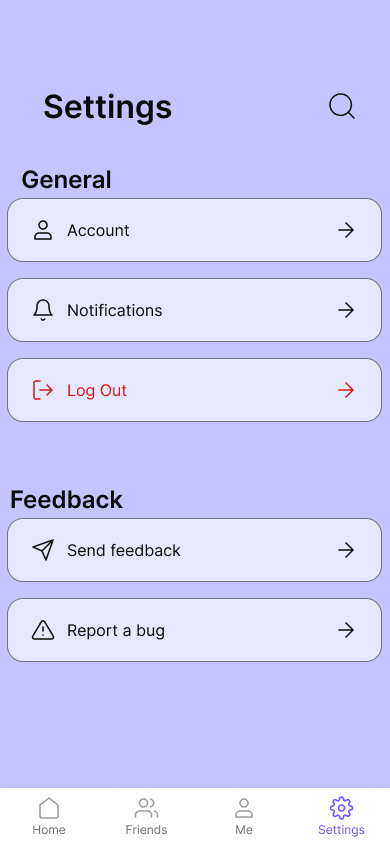
\includegraphics[width=\textwidth]{designSettings.png}}
        \caption{Settings}
    \end{subfigure}
    \hspace{0.5em}
    \noindent\begin{subfigure}[b]{0.23\textwidth}
        \centering
        \frame{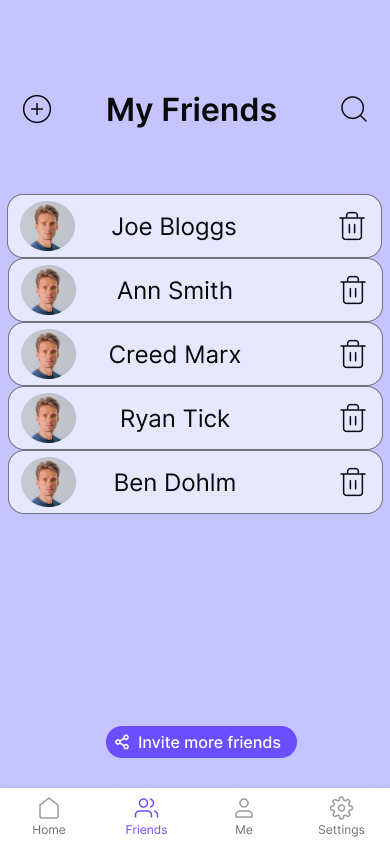
\includegraphics[width=\textwidth]{designFriends.png}}
        \caption{Friends}
    \end{subfigure}
    \hspace{0.5em}
    \noindent\begin{subfigure}[b]{0.23\textwidth}
        \centering
        \frame{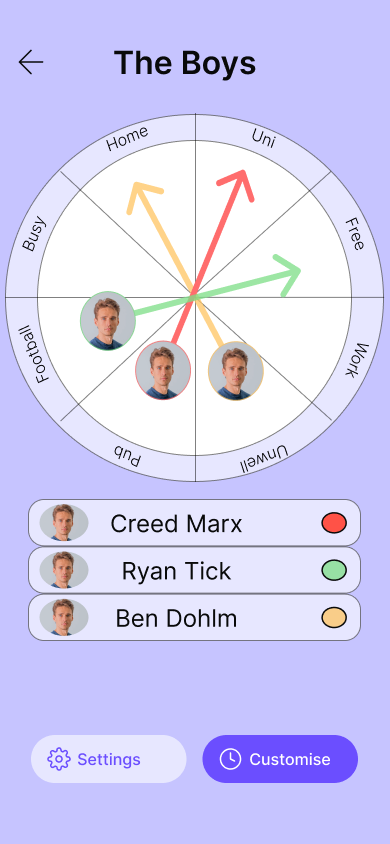
\includegraphics[width=\textwidth]{designClock.png}}
        \caption{Group}
    \end{subfigure}
    \hspace{0.5em}
    \noindent\begin{subfigure}[b]{0.23\textwidth}
        \centering
        \frame{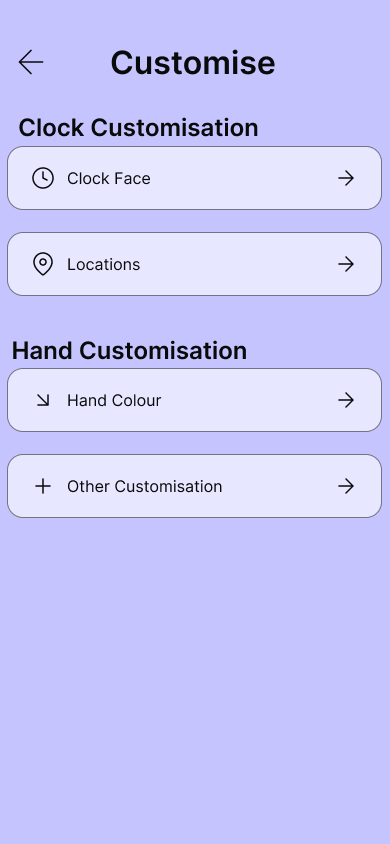
\includegraphics[width=\textwidth]{designGroupCust.png}}
        \caption{Group Customisation}
    \end{subfigure}
    \end{figure}
    \begin{figure}
    \ContinuedFloat
    \centering
    \noindent\begin{subfigure}[b]{0.23\textwidth}
        \centering
        \frame{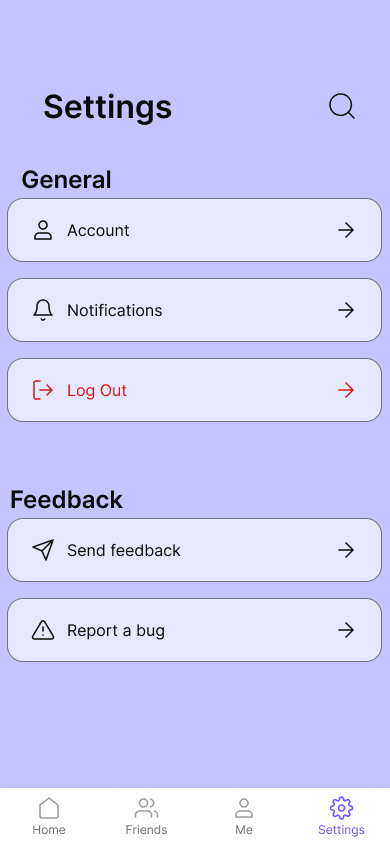
\includegraphics[width=\textwidth]{designGroupSett.png}}
        \caption{Group Settings}
    \end{subfigure}
    \hspace{0.5em}
    \noindent\begin{subfigure}[b]{0.23\textwidth}
        \centering
        \frame{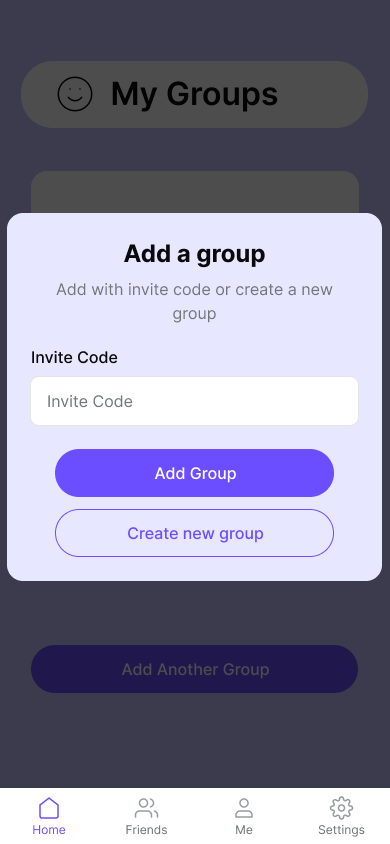
\includegraphics[width=\textwidth]{designAddGroup.png}}
        \caption{Add Group}
    \end{subfigure}
    \hspace{0.5em}
    \noindent\begin{subfigure}[b]{0.23\textwidth}
        \centering
        \frame{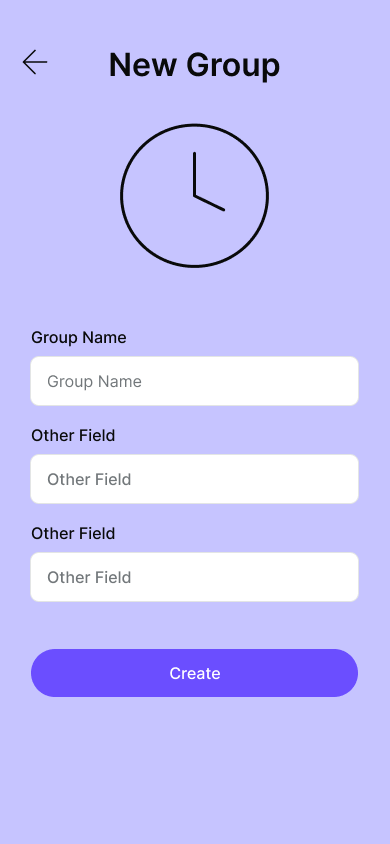
\includegraphics[width=\textwidth]{designNewGroup.png}}
        \caption{New Group }
    \end{subfigure}
    \hspace{0.5em}
    \noindent\begin{subfigure}[b]{0.23\textwidth}
        \centering
        \frame{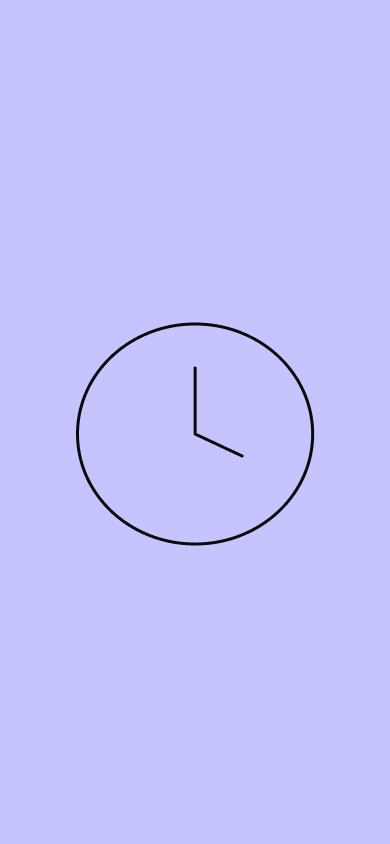
\includegraphics[width=\textwidth]{splash.png}}
        \caption{Splash}\label{splash}
    \end{subfigure}
    \caption{Figma Designs}
\end{figure}
\FloatBarrier


\section{Application User Interface}\label{appendix:appScreens}
\begin{figure}[!htbp]
    \centering
    \noindent\begin{subfigure}[b]{0.23\textwidth}
        \centering
        \frame{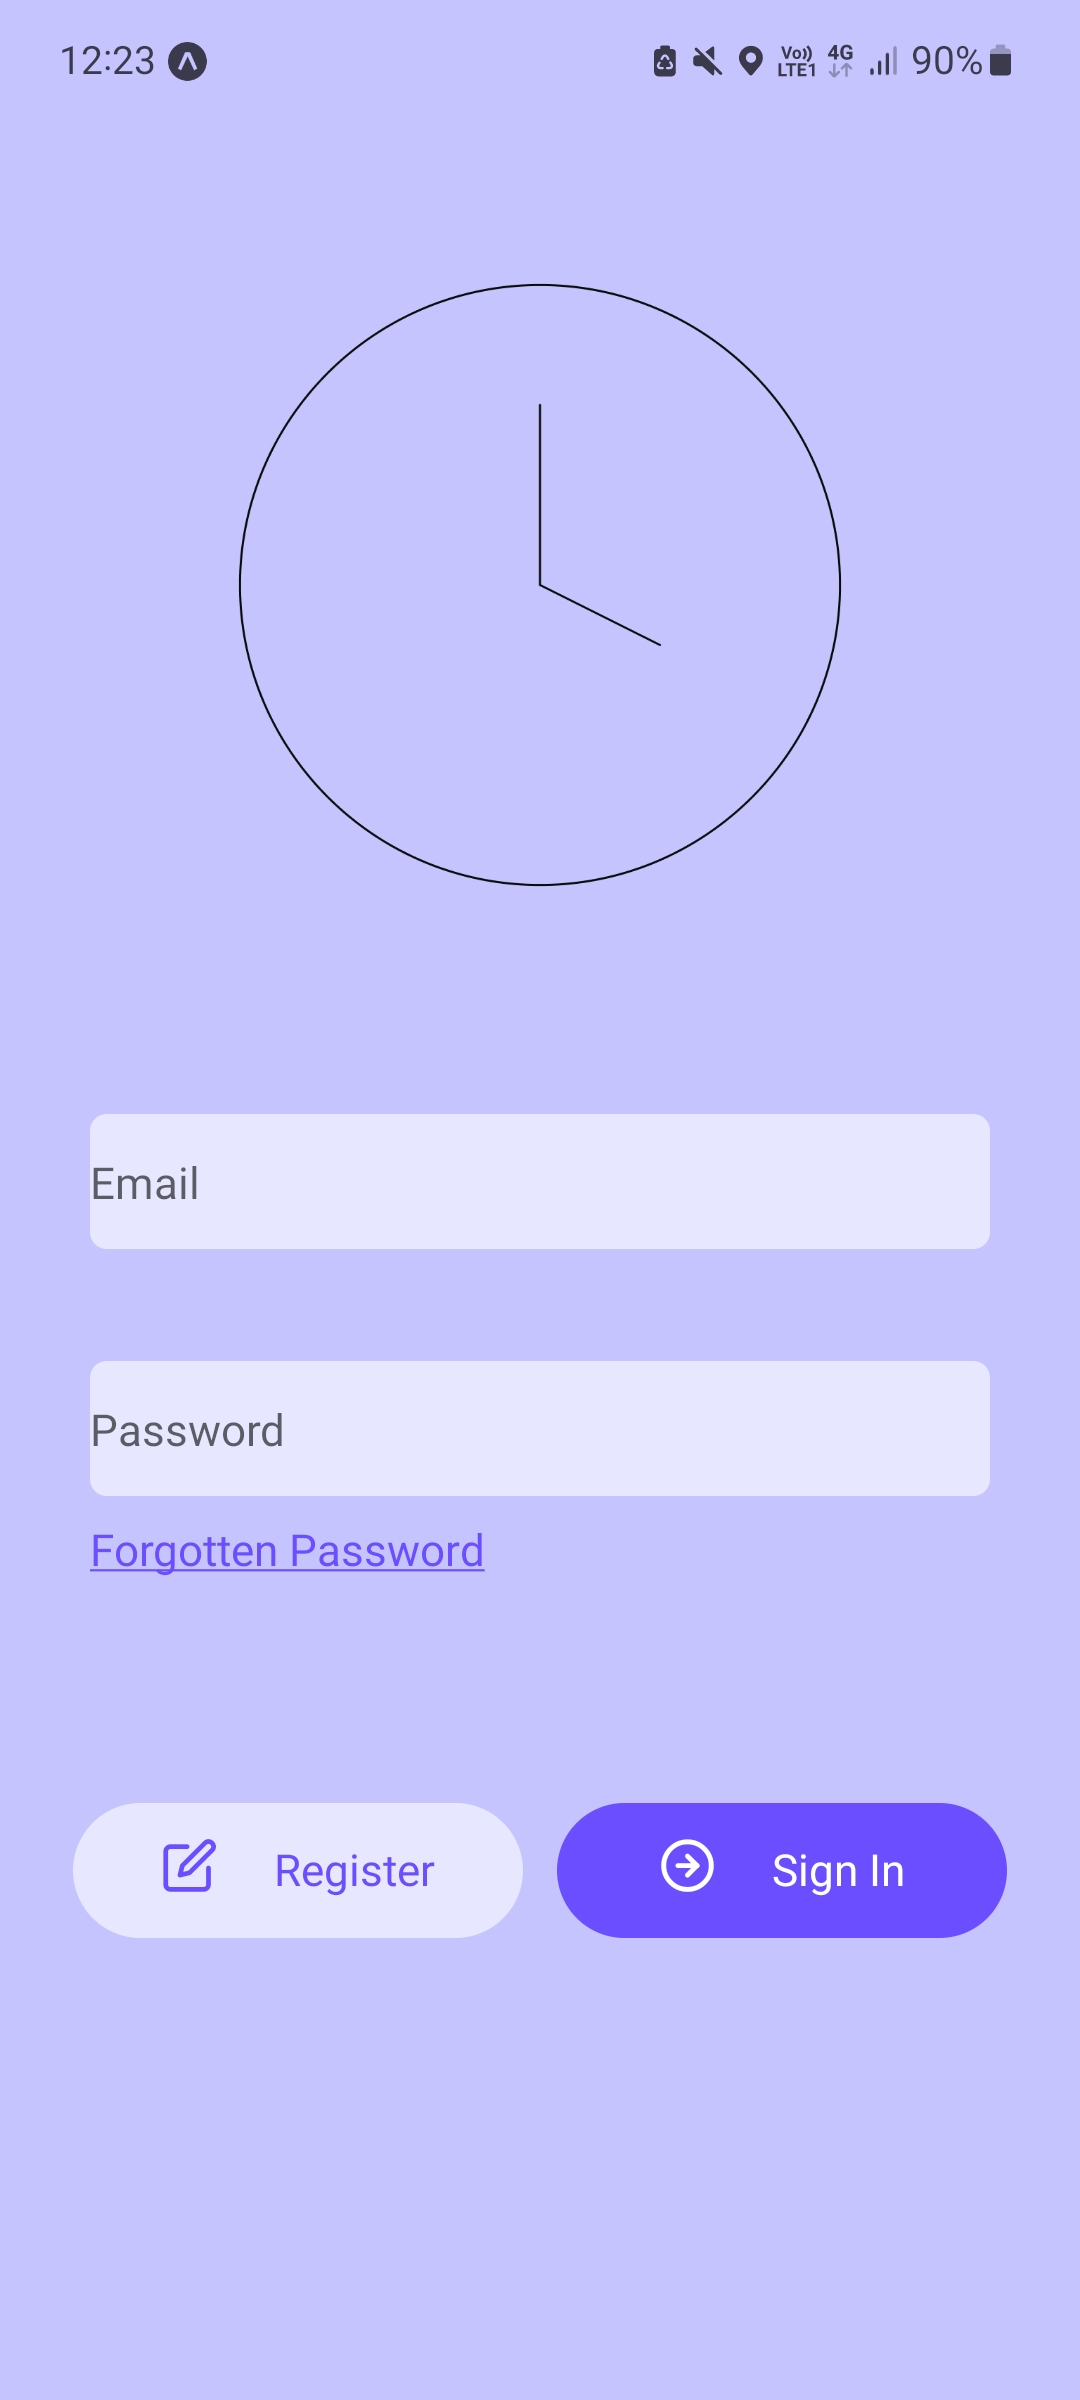
\includegraphics[width=\textwidth]{signIn.jpg}}
        \caption{Sign In}
    \end{subfigure}
    \hspace{0.5em}
    \noindent\begin{subfigure}[b]{0.23\textwidth}
        \centering
        \frame{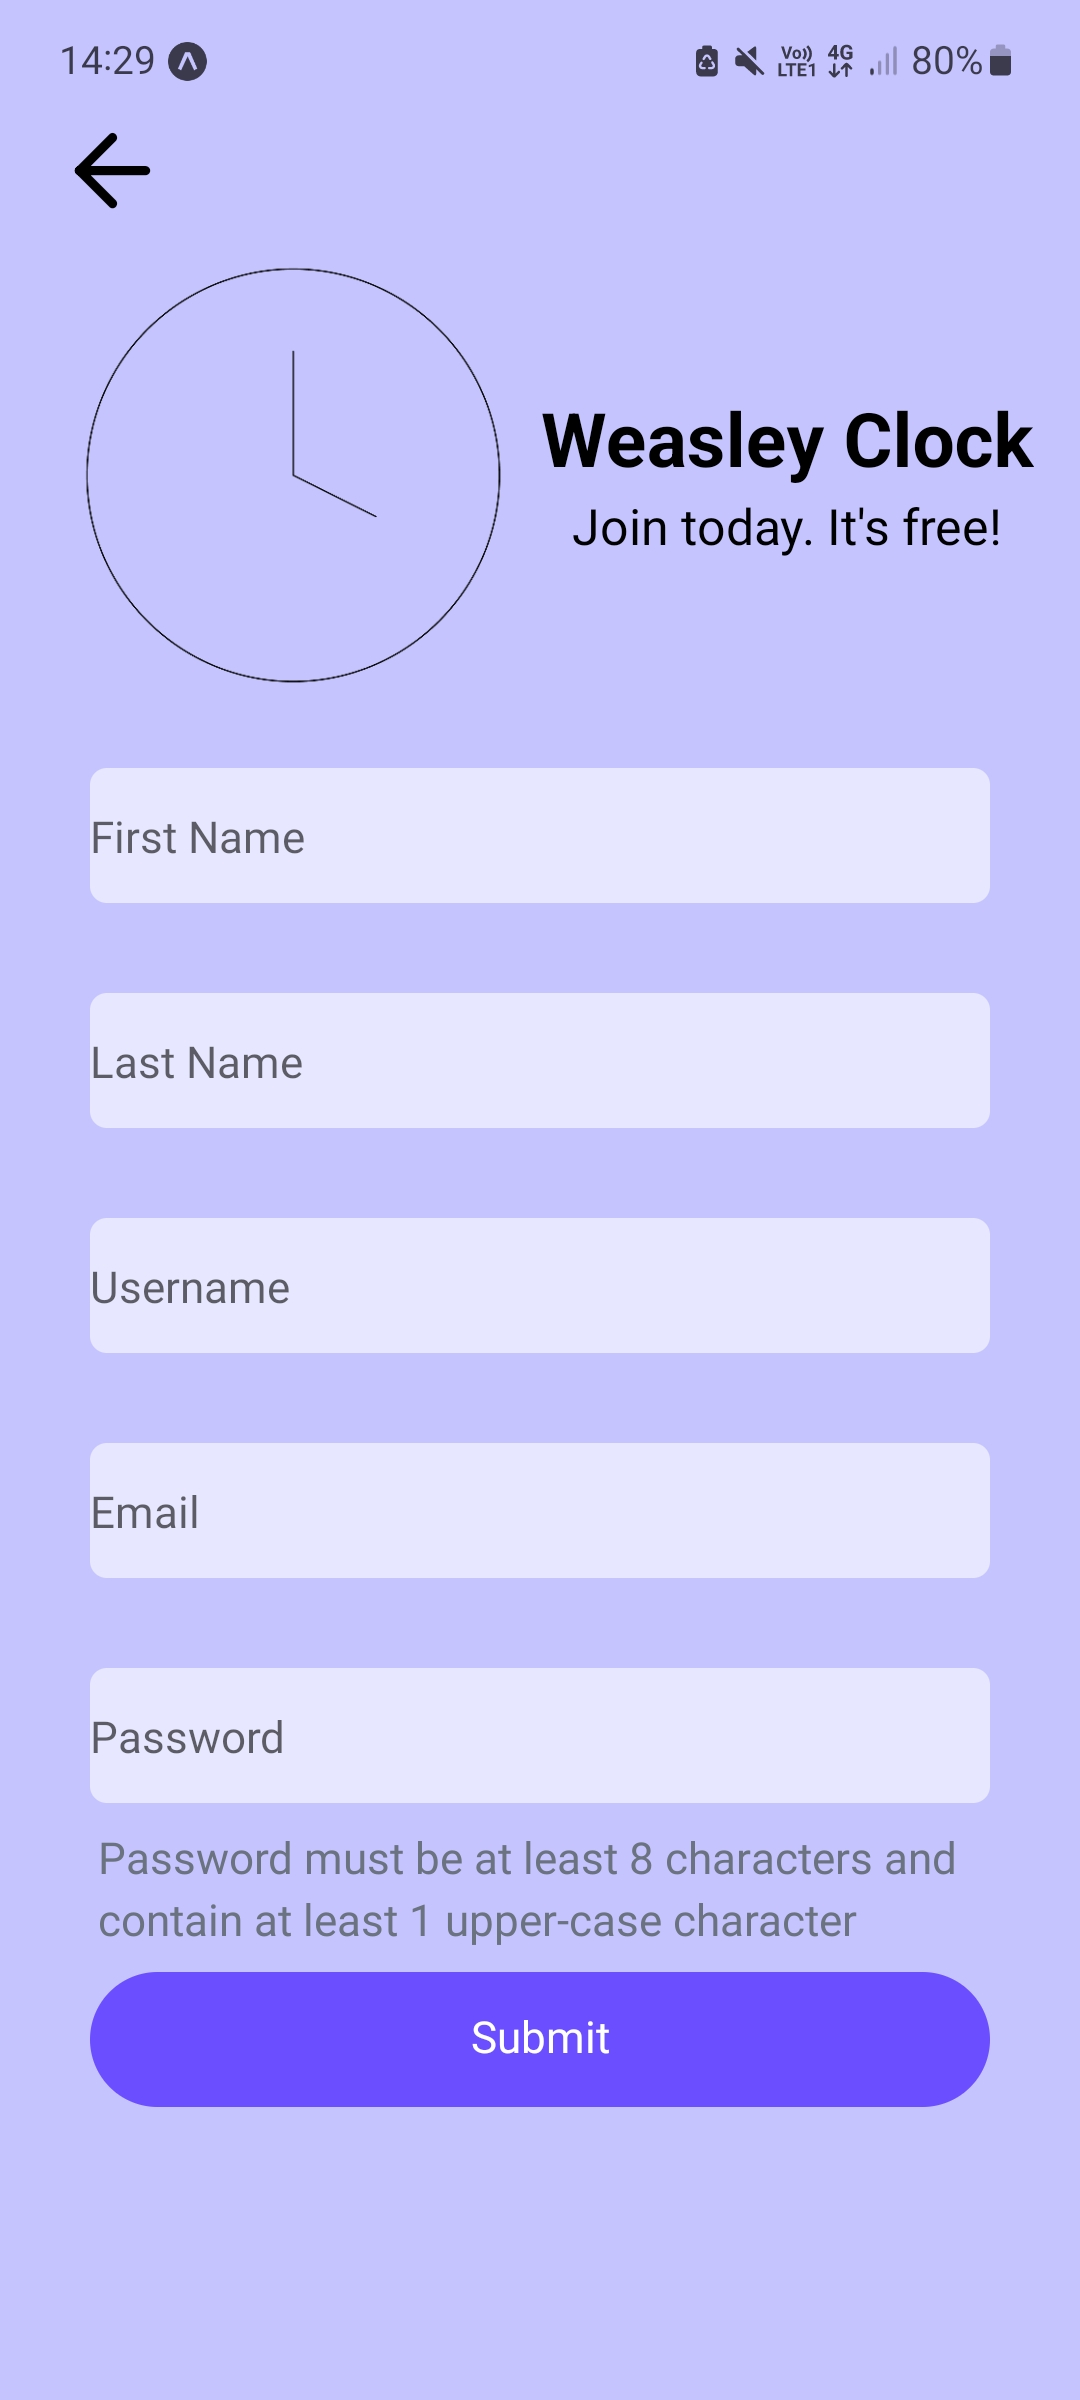
\includegraphics[width=\textwidth]{register.jpg}}
        \caption{Register}
    \end{subfigure}
    \hspace{0.5em}
    \noindent\begin{subfigure}[b]{0.23\textwidth}
        \centering
        \frame{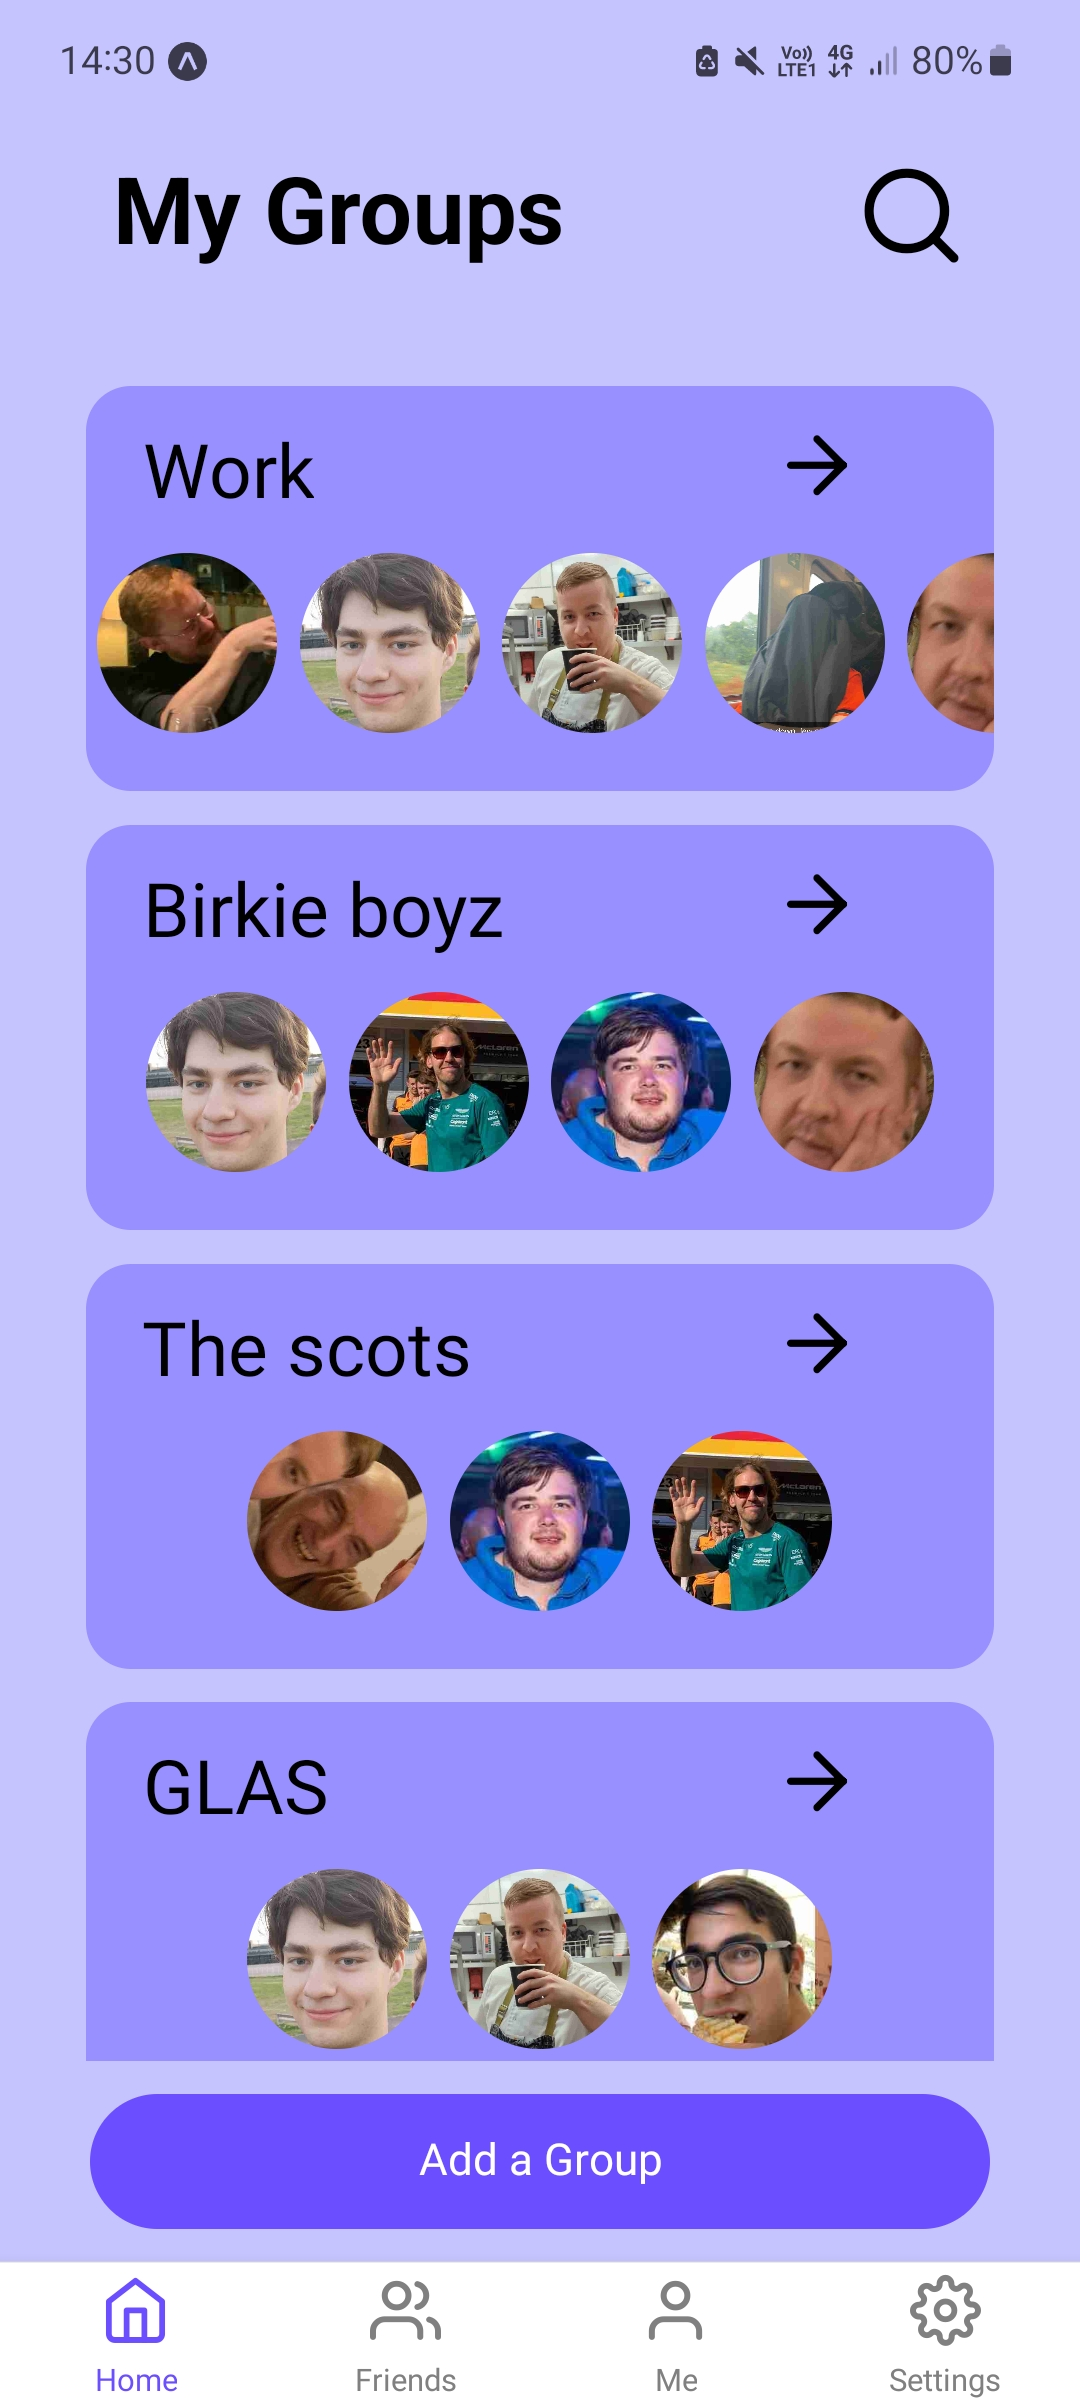
\includegraphics[width=\textwidth]{home.jpg}}
        \caption{Home}
    \end{subfigure}
    \hspace{0.5em}
    \noindent\begin{subfigure}[b]{0.23\textwidth}
        \centering
        \frame{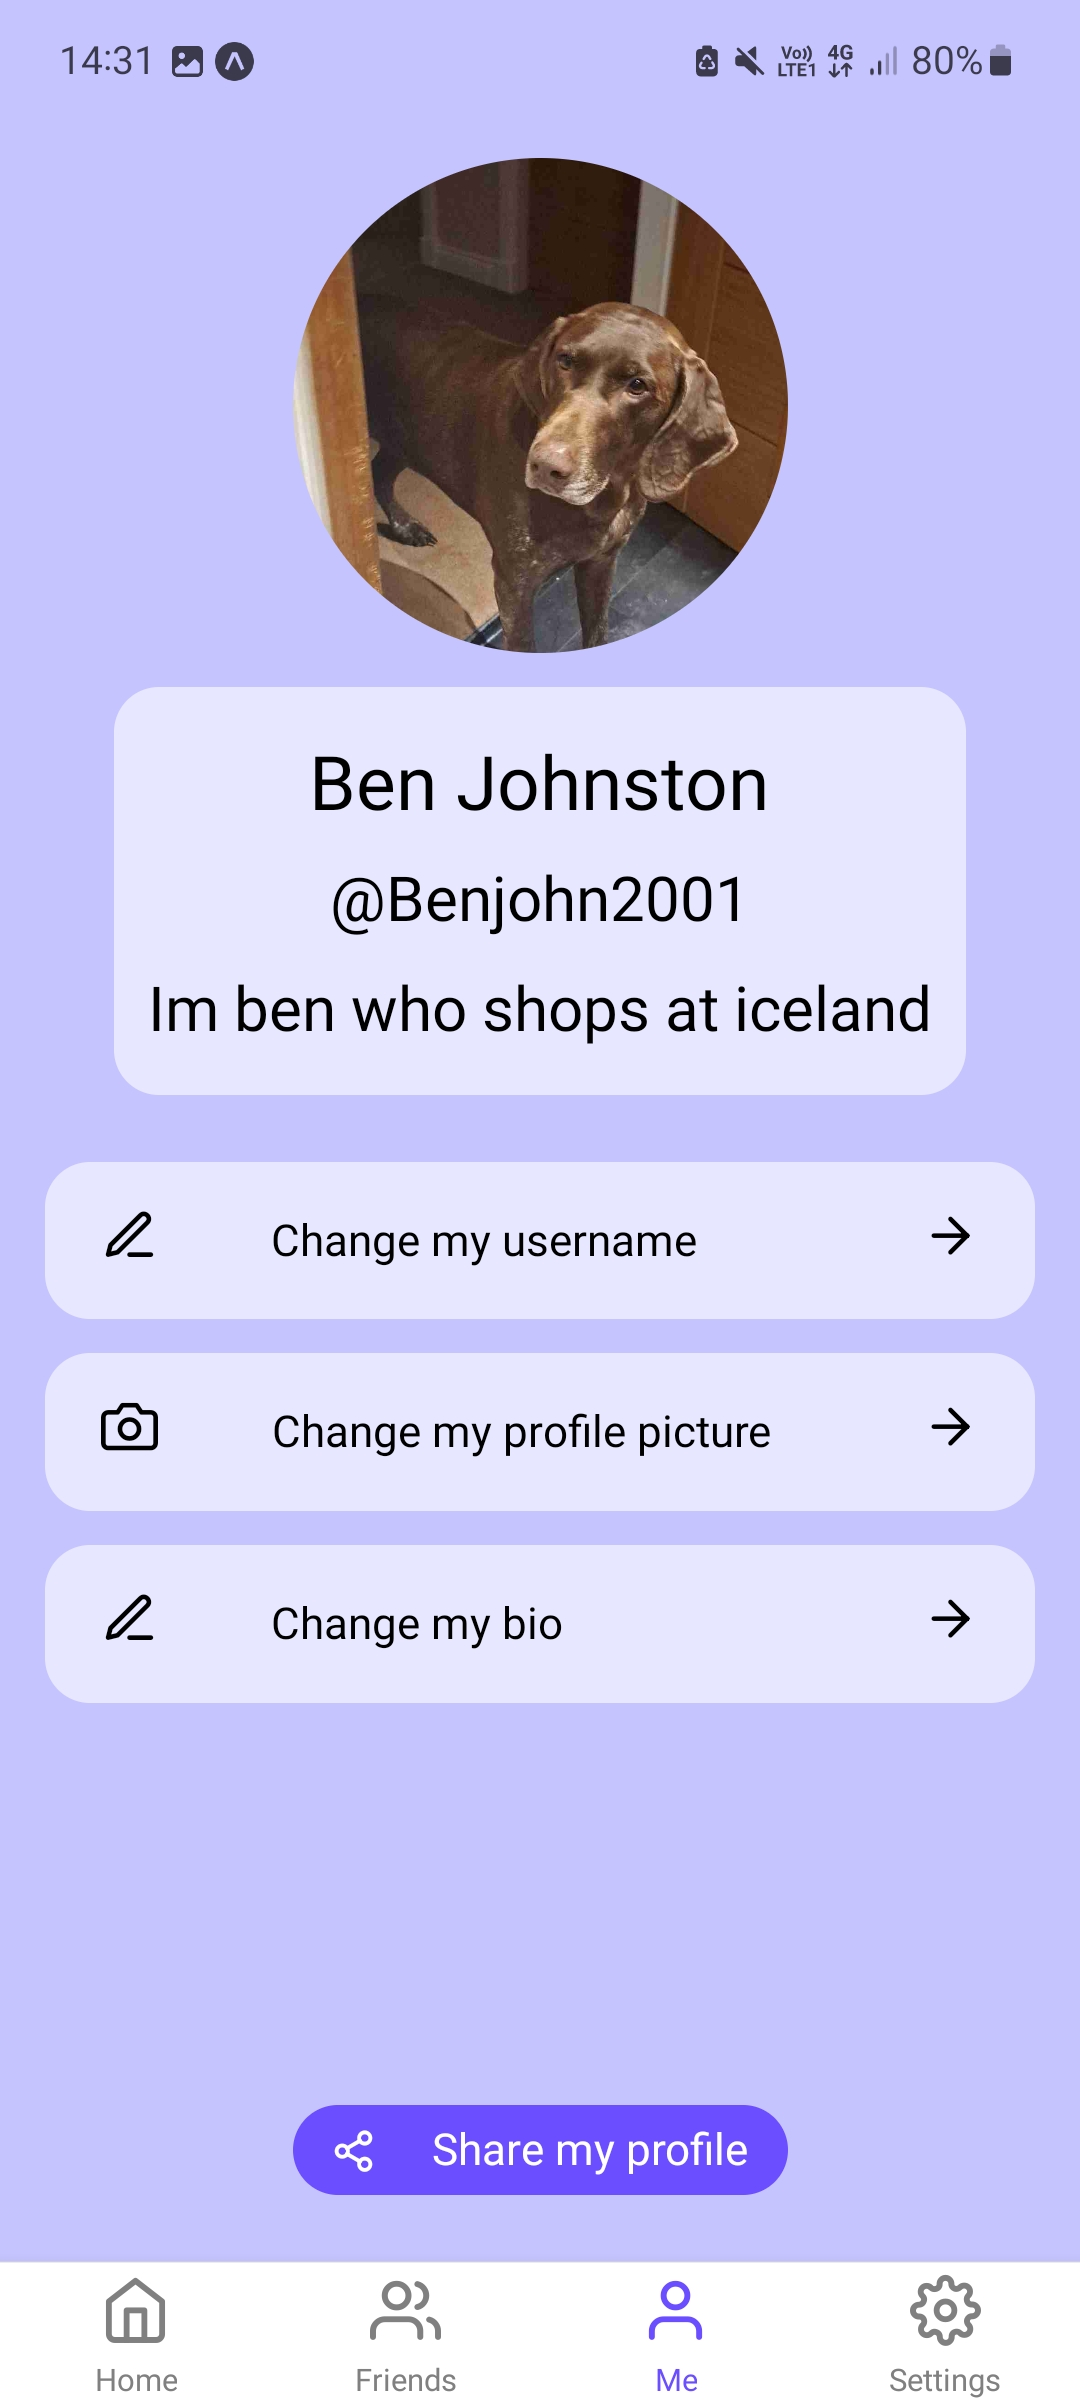
\includegraphics[width=\textwidth]{myProfile.jpg}}
        \caption{User Profile}
    \end{subfigure}
    \end{figure}
    \FloatBarrier
    \begin{figure}
    \ContinuedFloat
    \centering
    \noindent\begin{subfigure}[b]{0.23\textwidth}
        \centering
        \frame{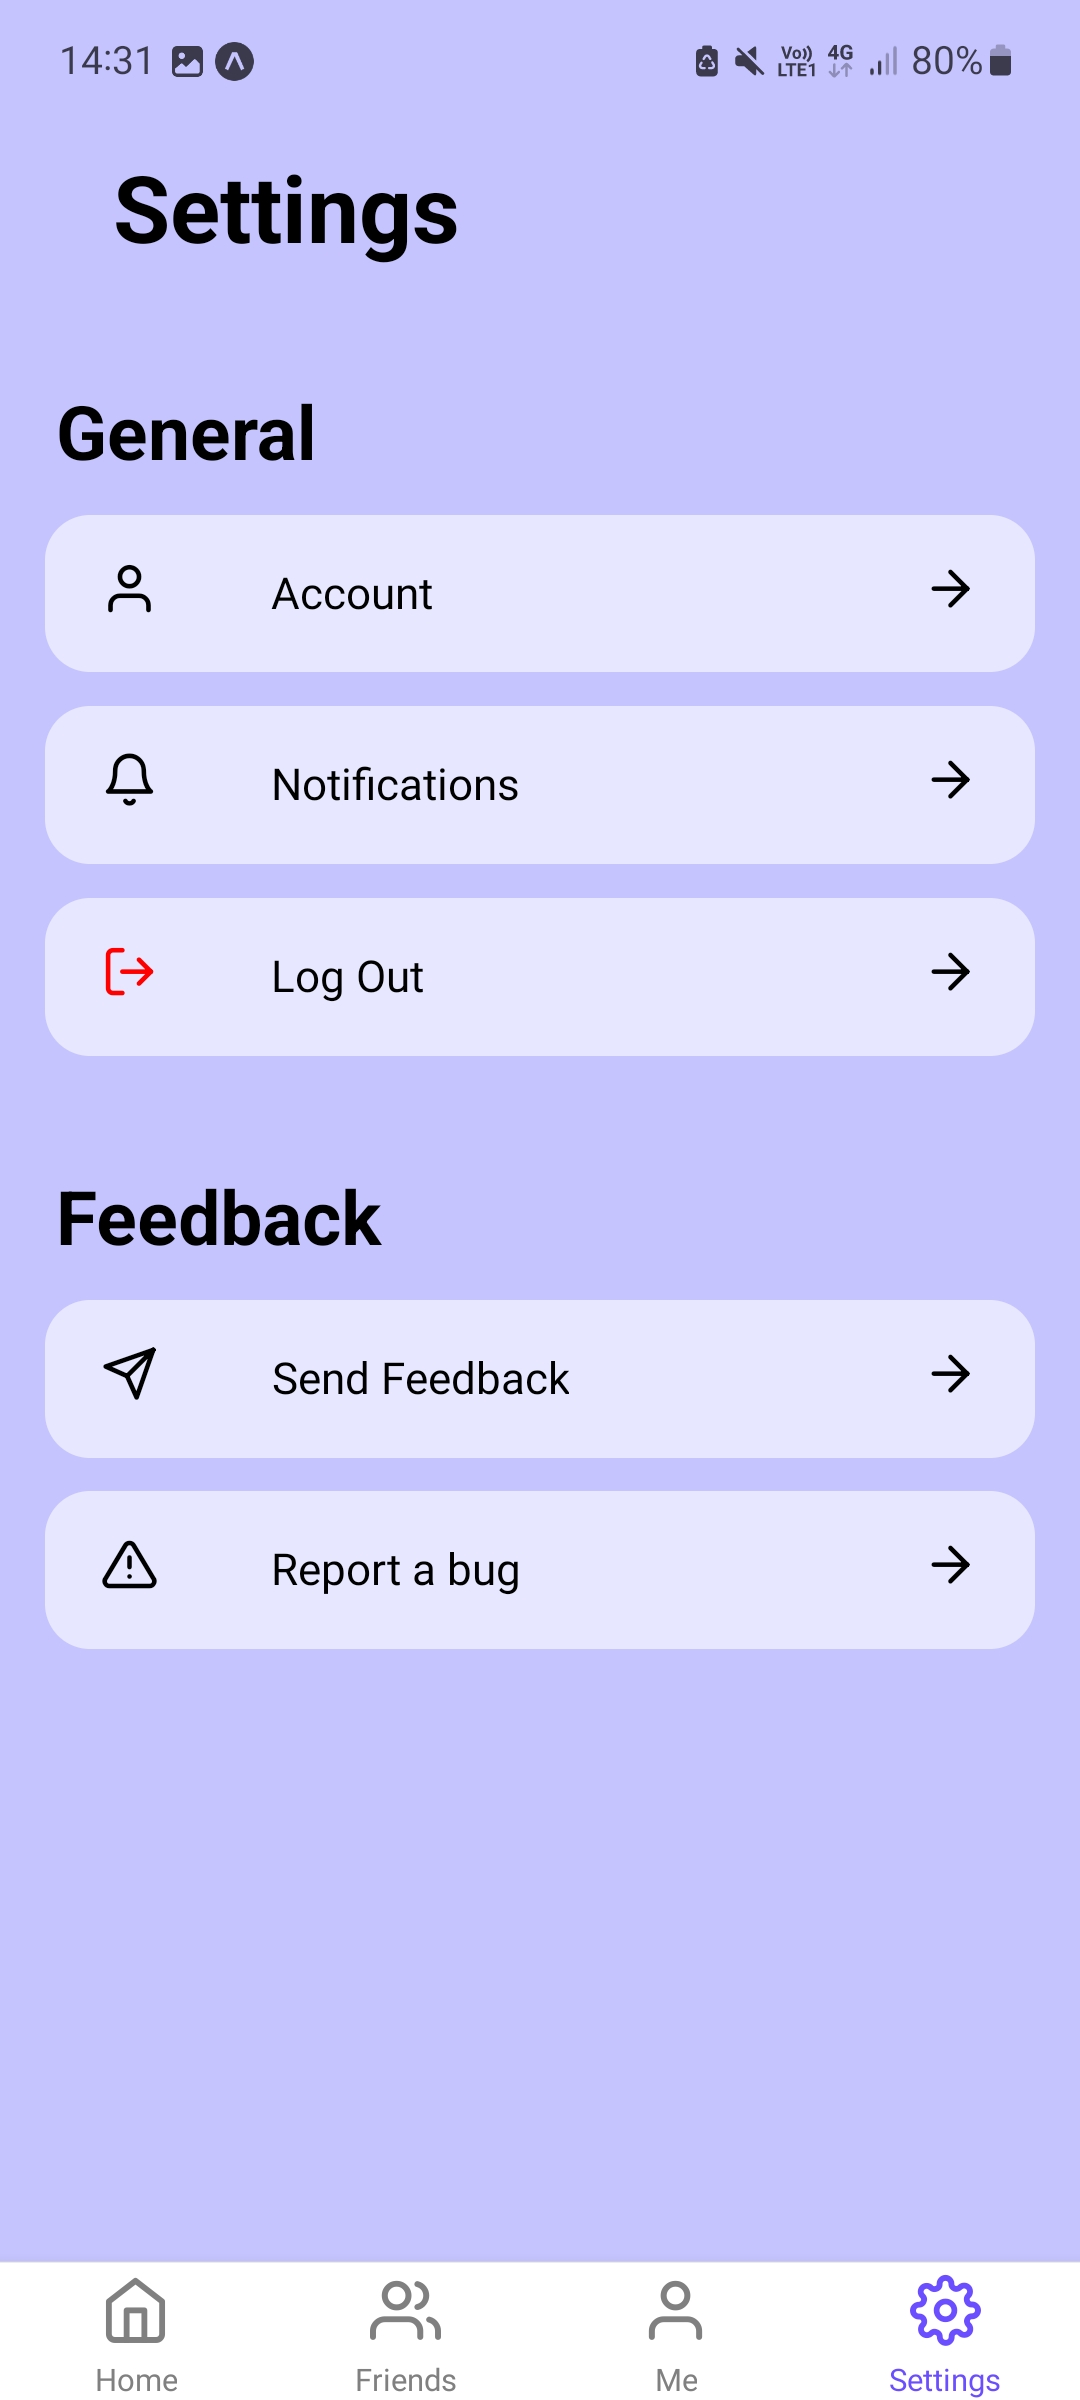
\includegraphics[width=\textwidth]{settings.jpg}}
        \caption{Settings}
    \end{subfigure}
    \hspace{0.5em}
    \noindent\begin{subfigure}[b]{0.23\textwidth}
        \centering
        \frame{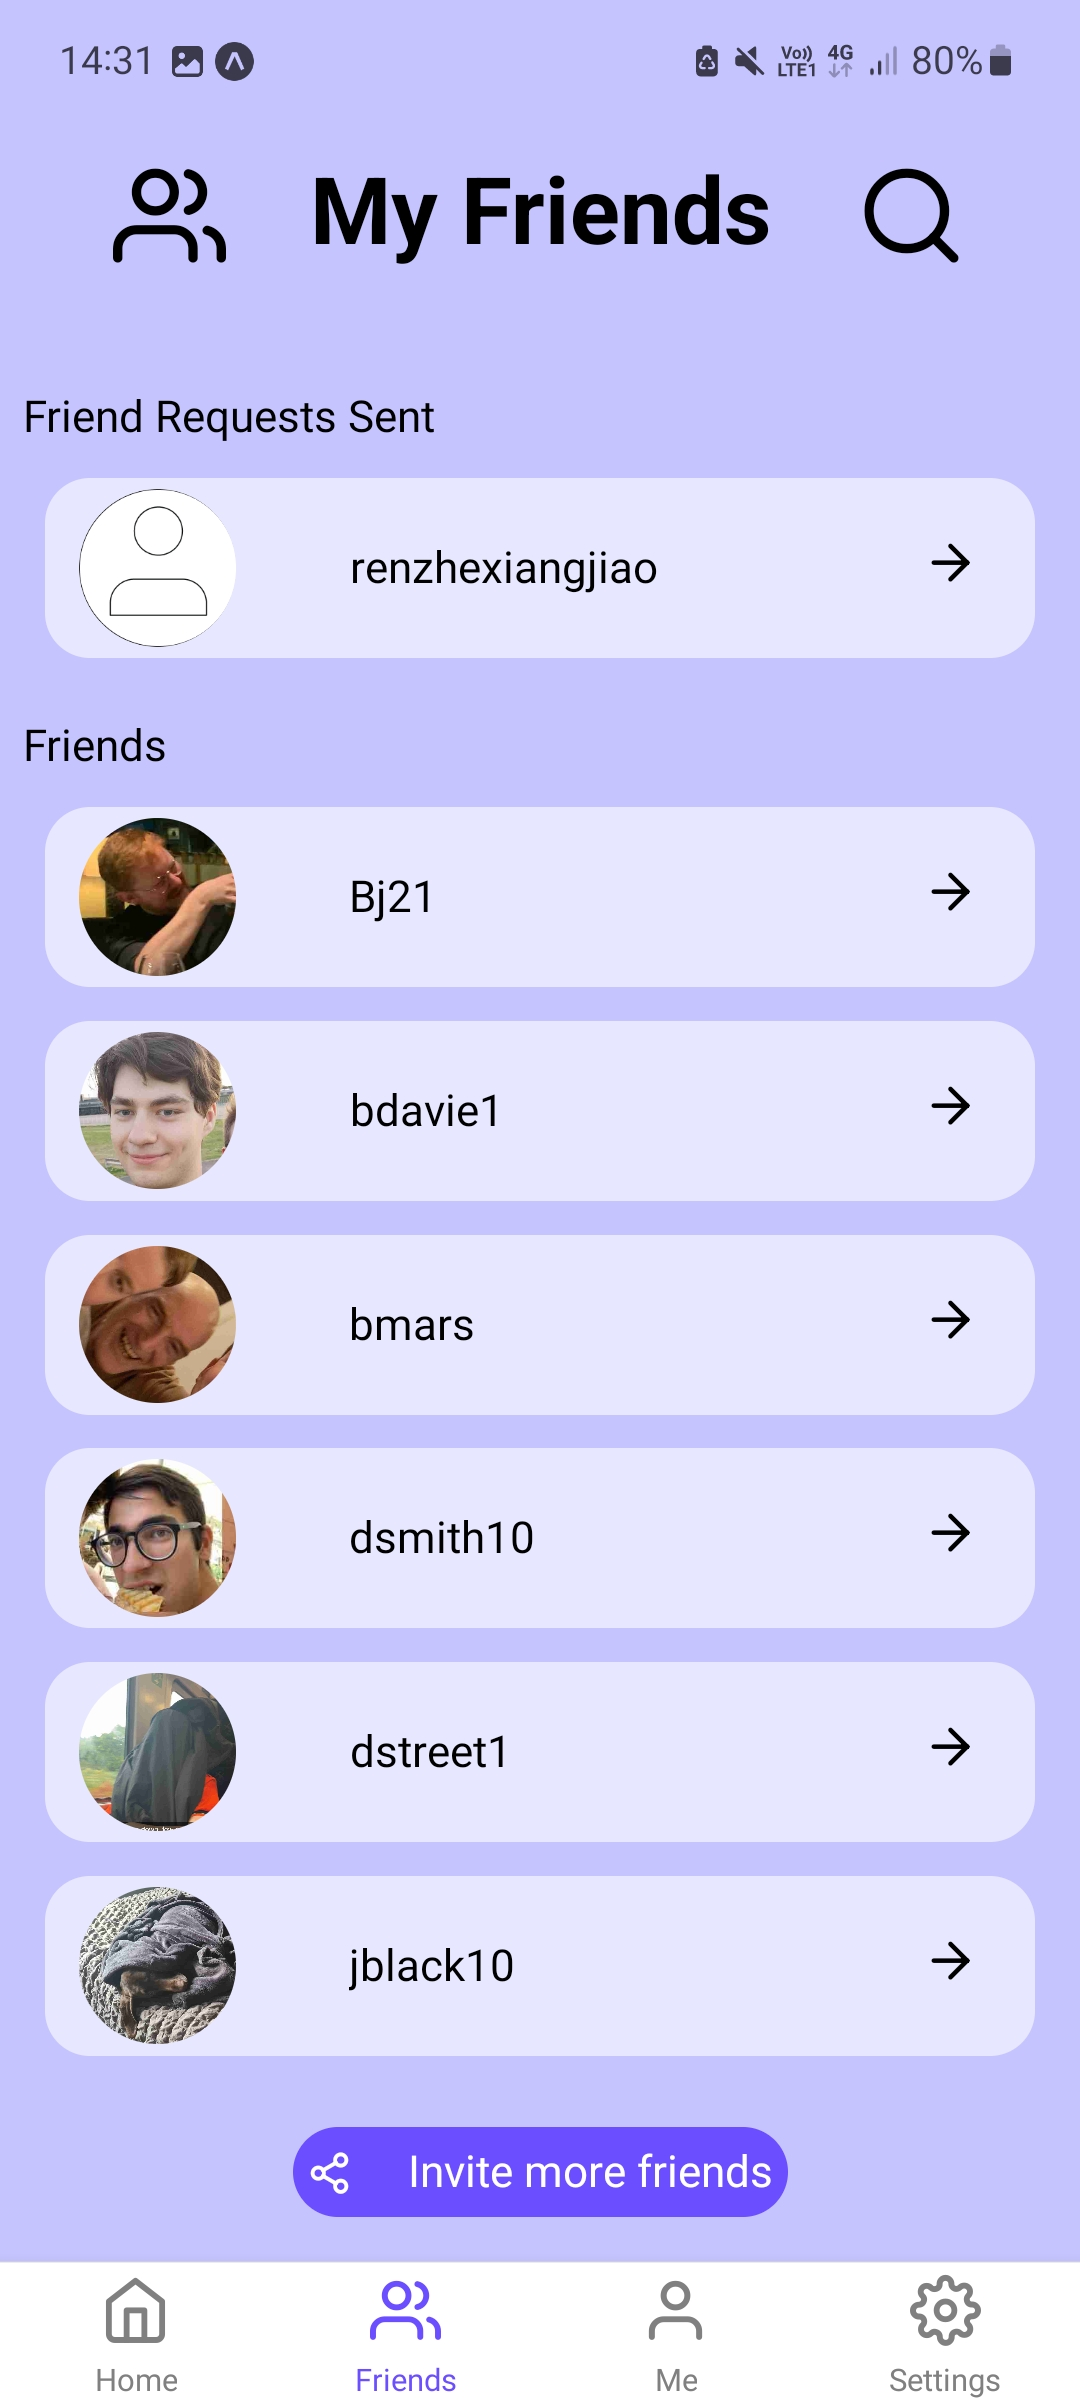
\includegraphics[width=\textwidth]{friendsList.jpg}}
        \caption{Friends List}
    \end{subfigure}
    \hspace{0.5em}
    \noindent\begin{subfigure}[b]{0.23\textwidth}
        \centering
        \frame{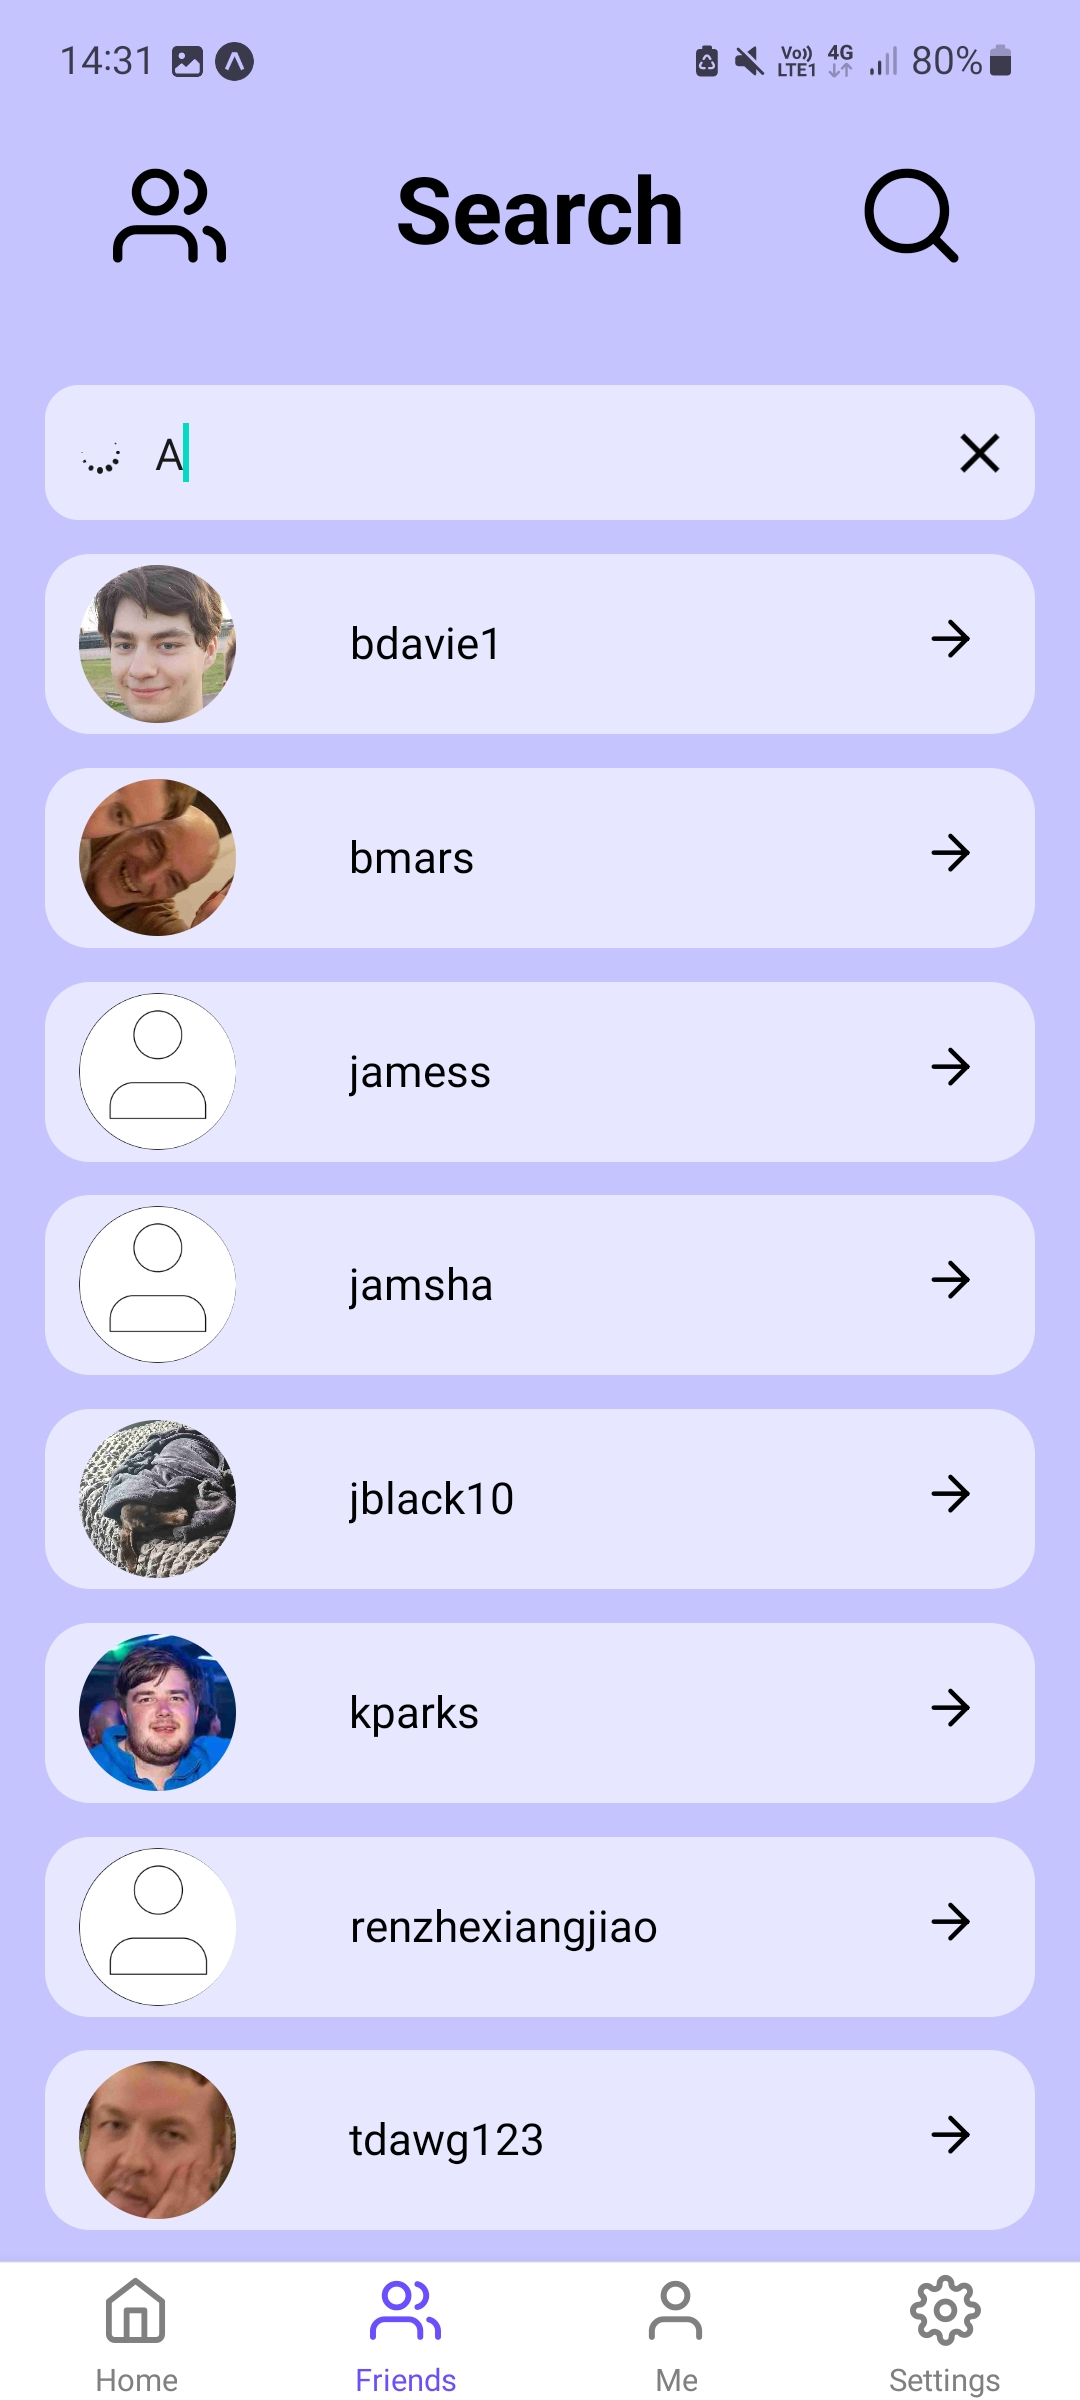
\includegraphics[width=\textwidth]{searchFriends.jpg}}
        \caption{Friends Search}
    \end{subfigure}
    \hspace{0.5em}
    \noindent\begin{subfigure}[b]{0.23\textwidth}
        \centering
        \frame{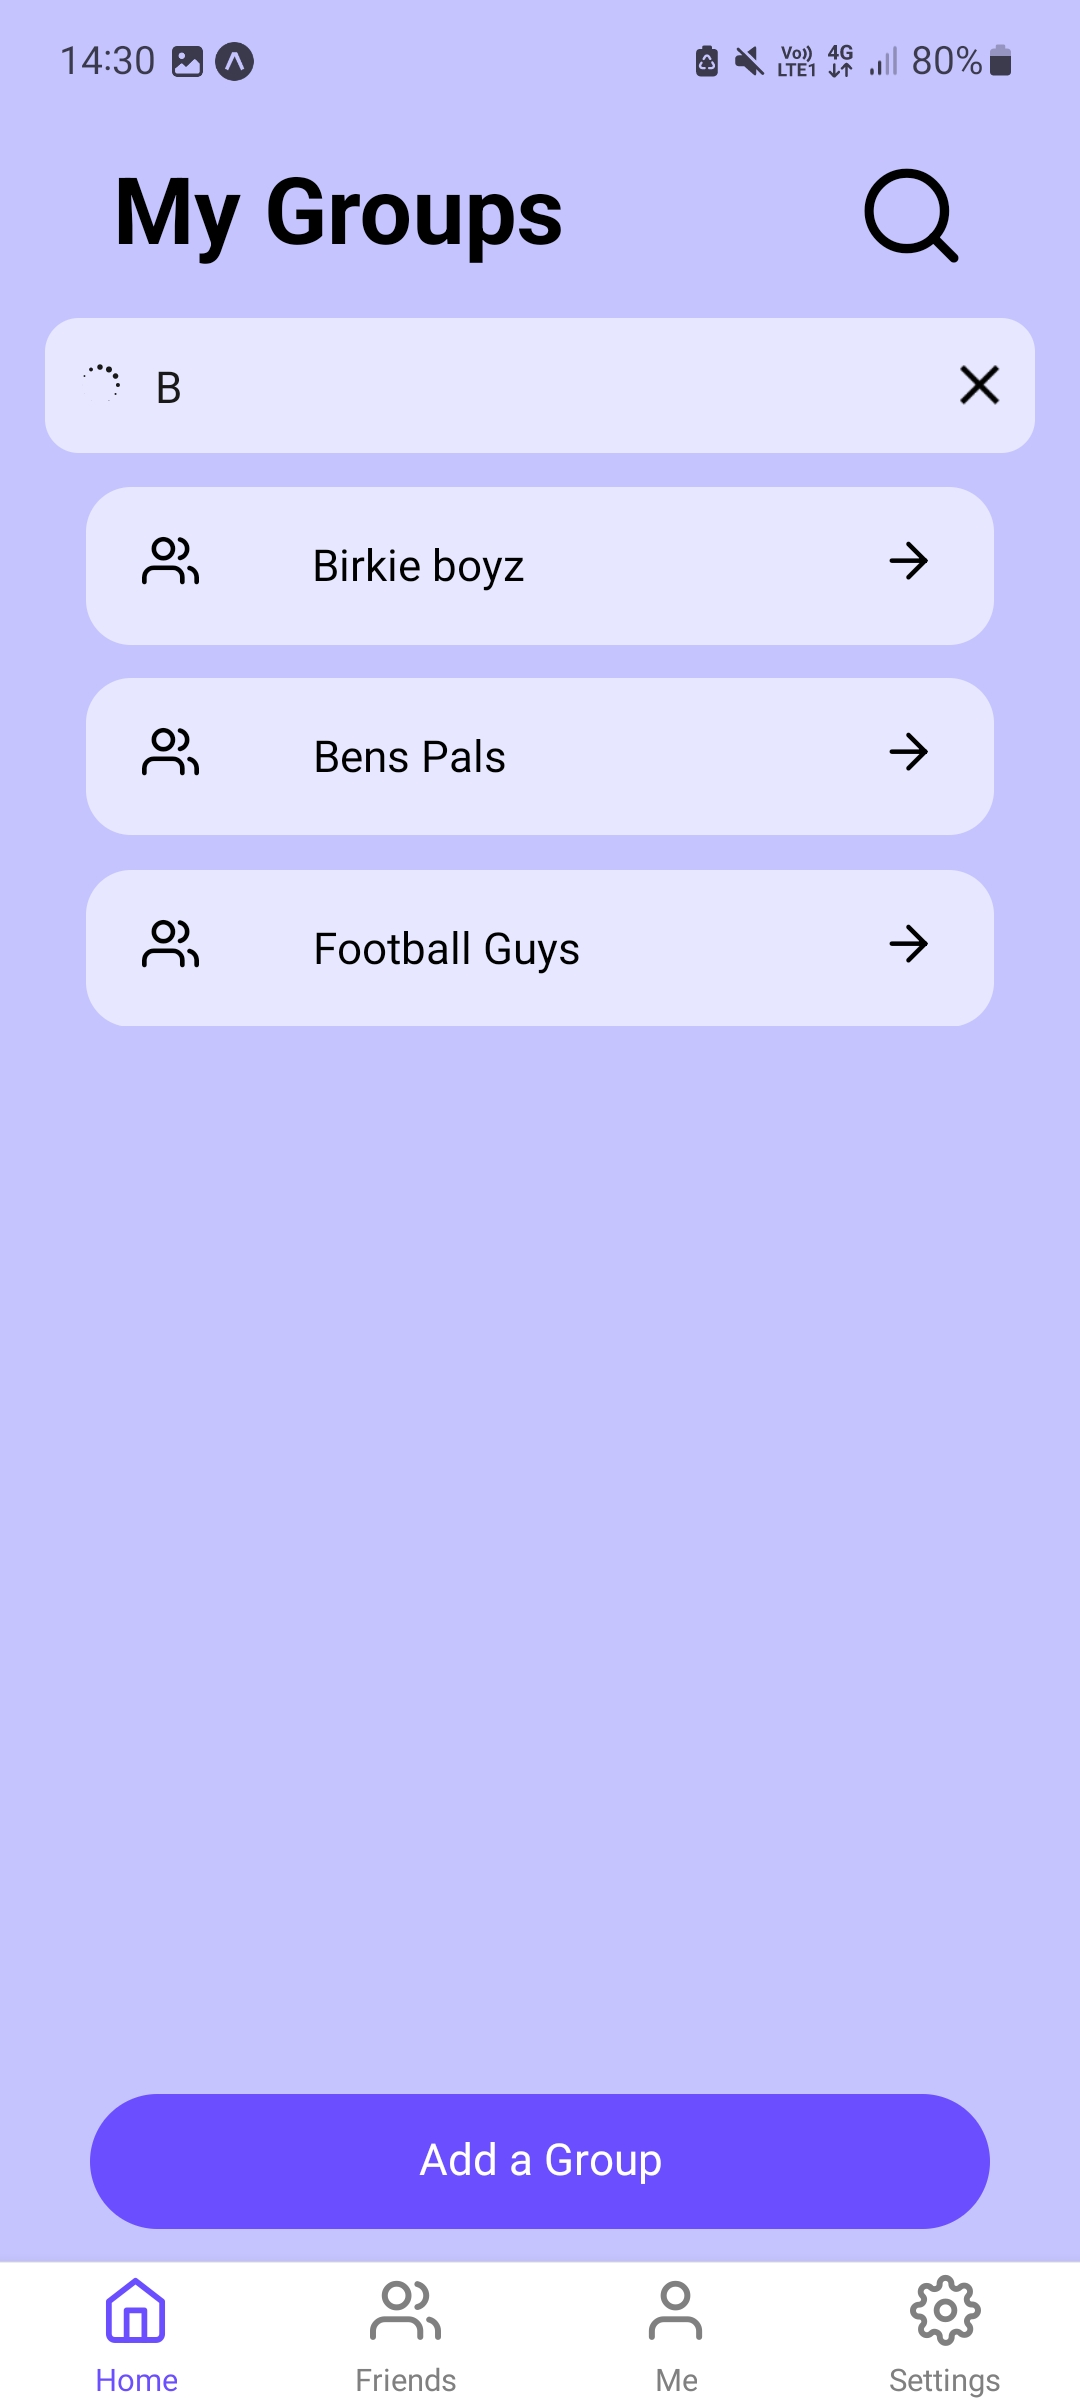
\includegraphics[width=\textwidth]{searchGroups.jpg}}
        \caption{Groups Search}
    \end{subfigure}
    \vskip\baselineskip
    \noindent\begin{subfigure}[b]{0.23\textwidth}
        \centering
        \frame{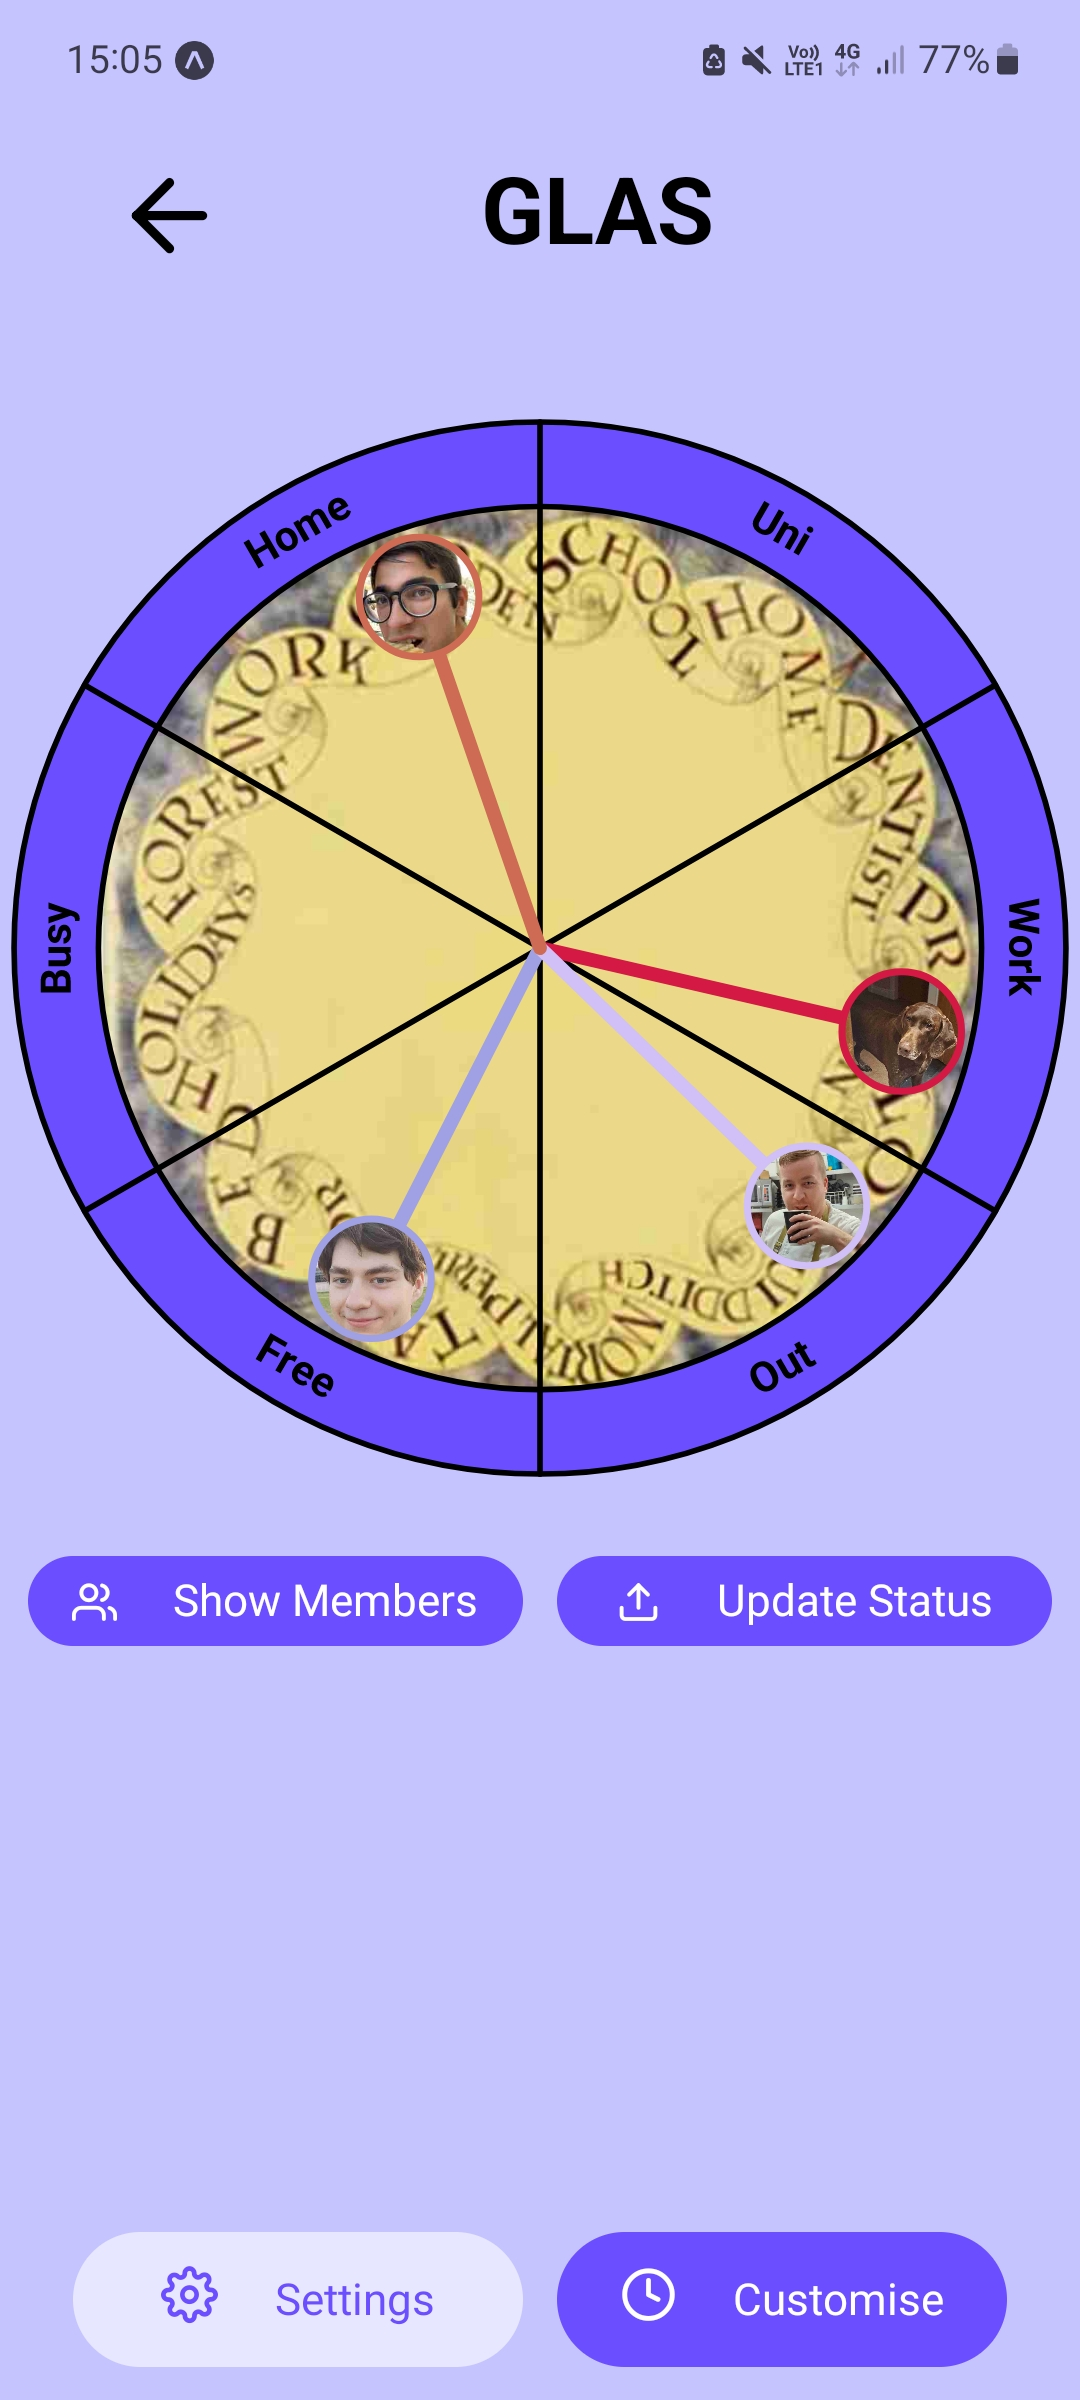
\includegraphics[width=\textwidth]{clock.jpg}}
        \caption{Group}
    \end{subfigure}
    \hspace{0.5em}
    \noindent\begin{subfigure}[b]{0.23\textwidth}
        \centering
        \frame{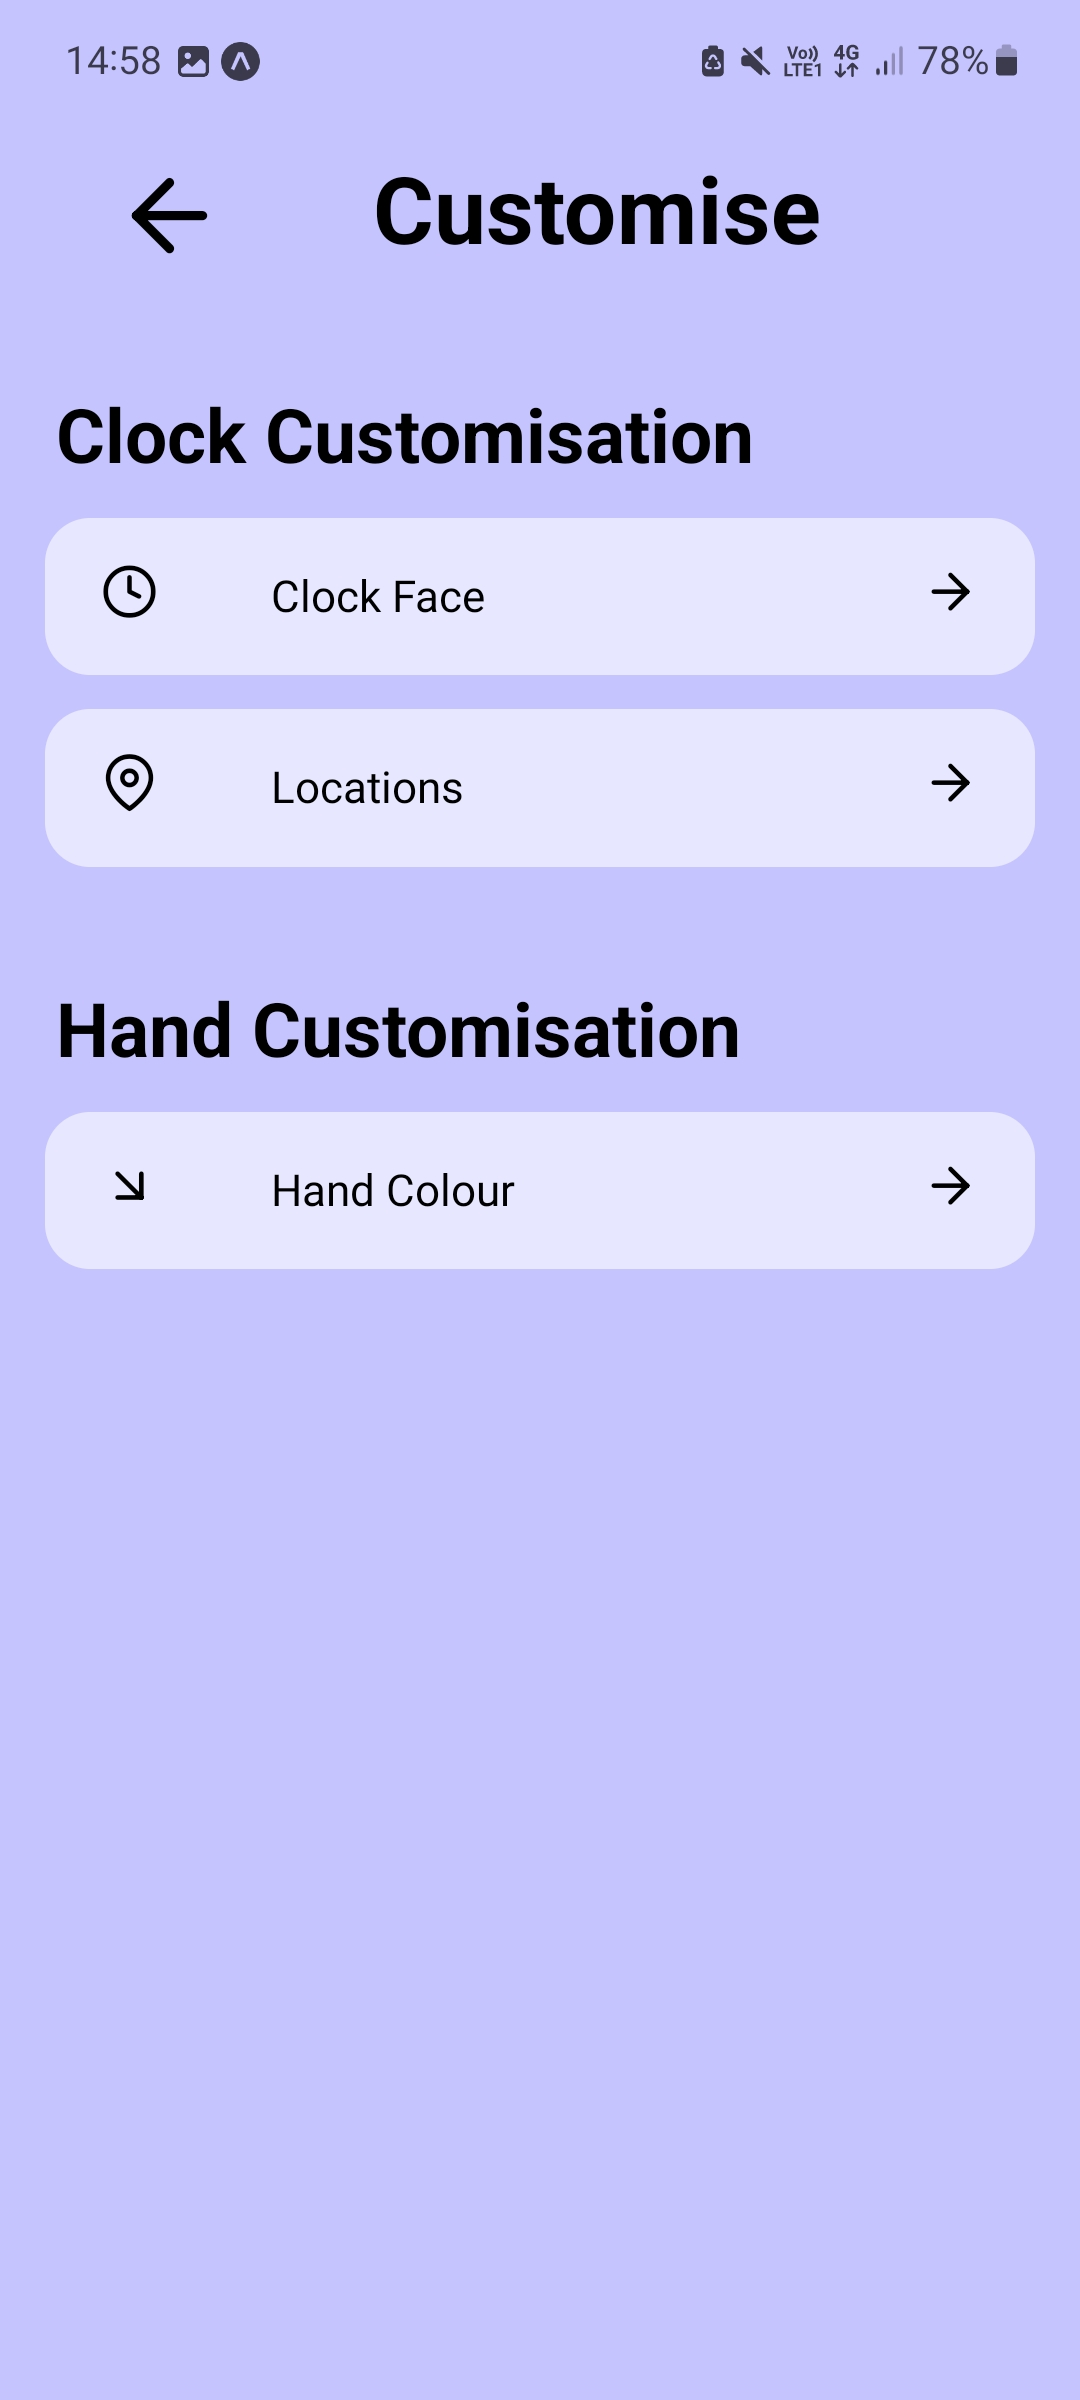
\includegraphics[width=\textwidth]{groupCustomisation.jpg}}
        \caption{Group Customisation}
    \end{subfigure}
    \hspace{0.5em}
    \noindent\begin{subfigure}[b]{0.23\textwidth}
        \centering
        \frame{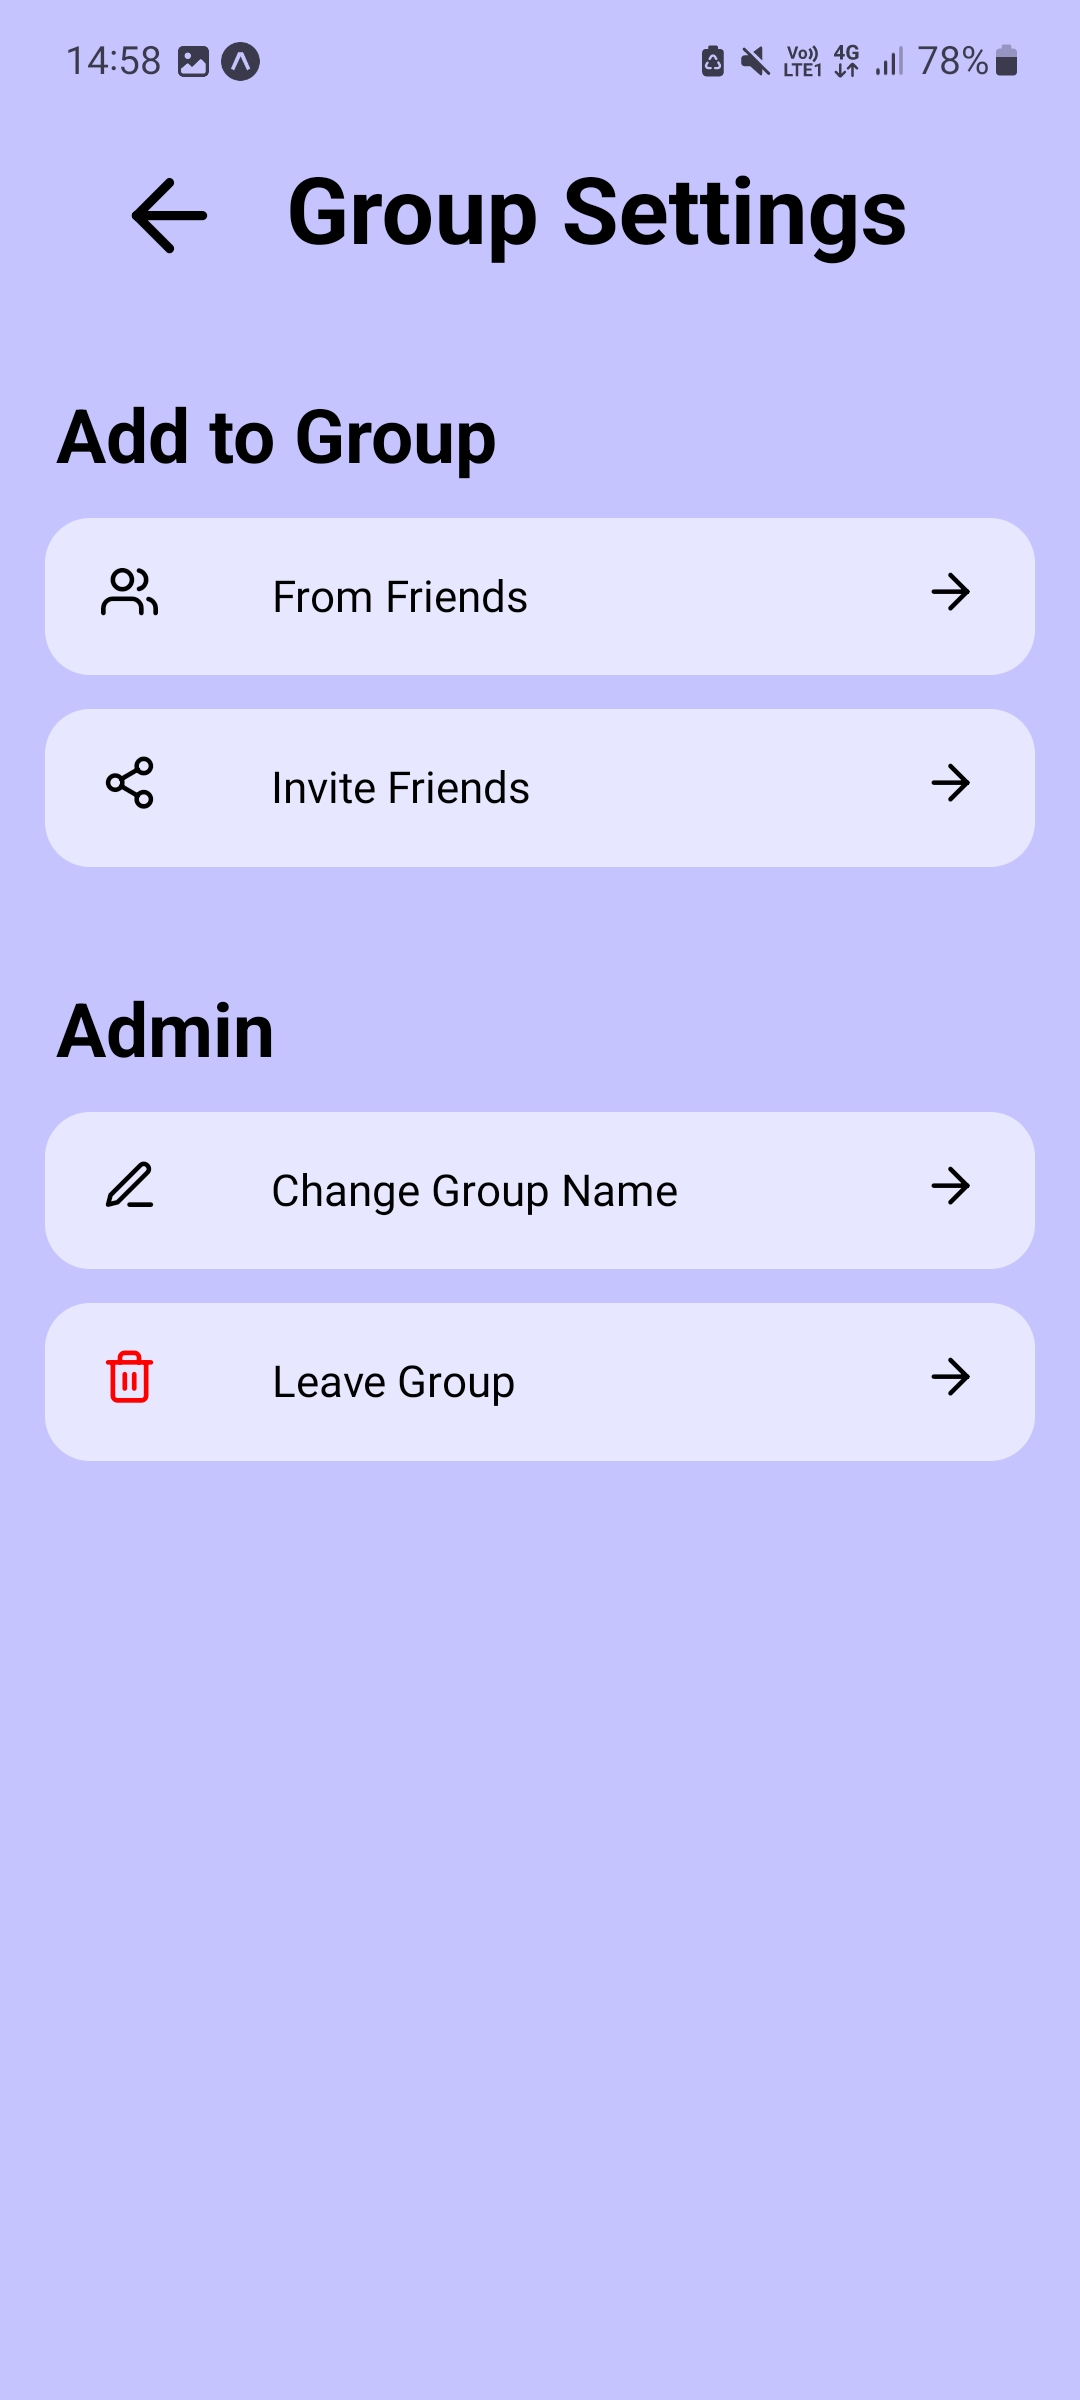
\includegraphics[width=\textwidth]{groupSettings.jpg}}
        \caption{Group Settings}
    \end{subfigure}
    \hspace{0.5em}
    \noindent\begin{subfigure}[b]{0.23\textwidth}
        \centering
        \frame{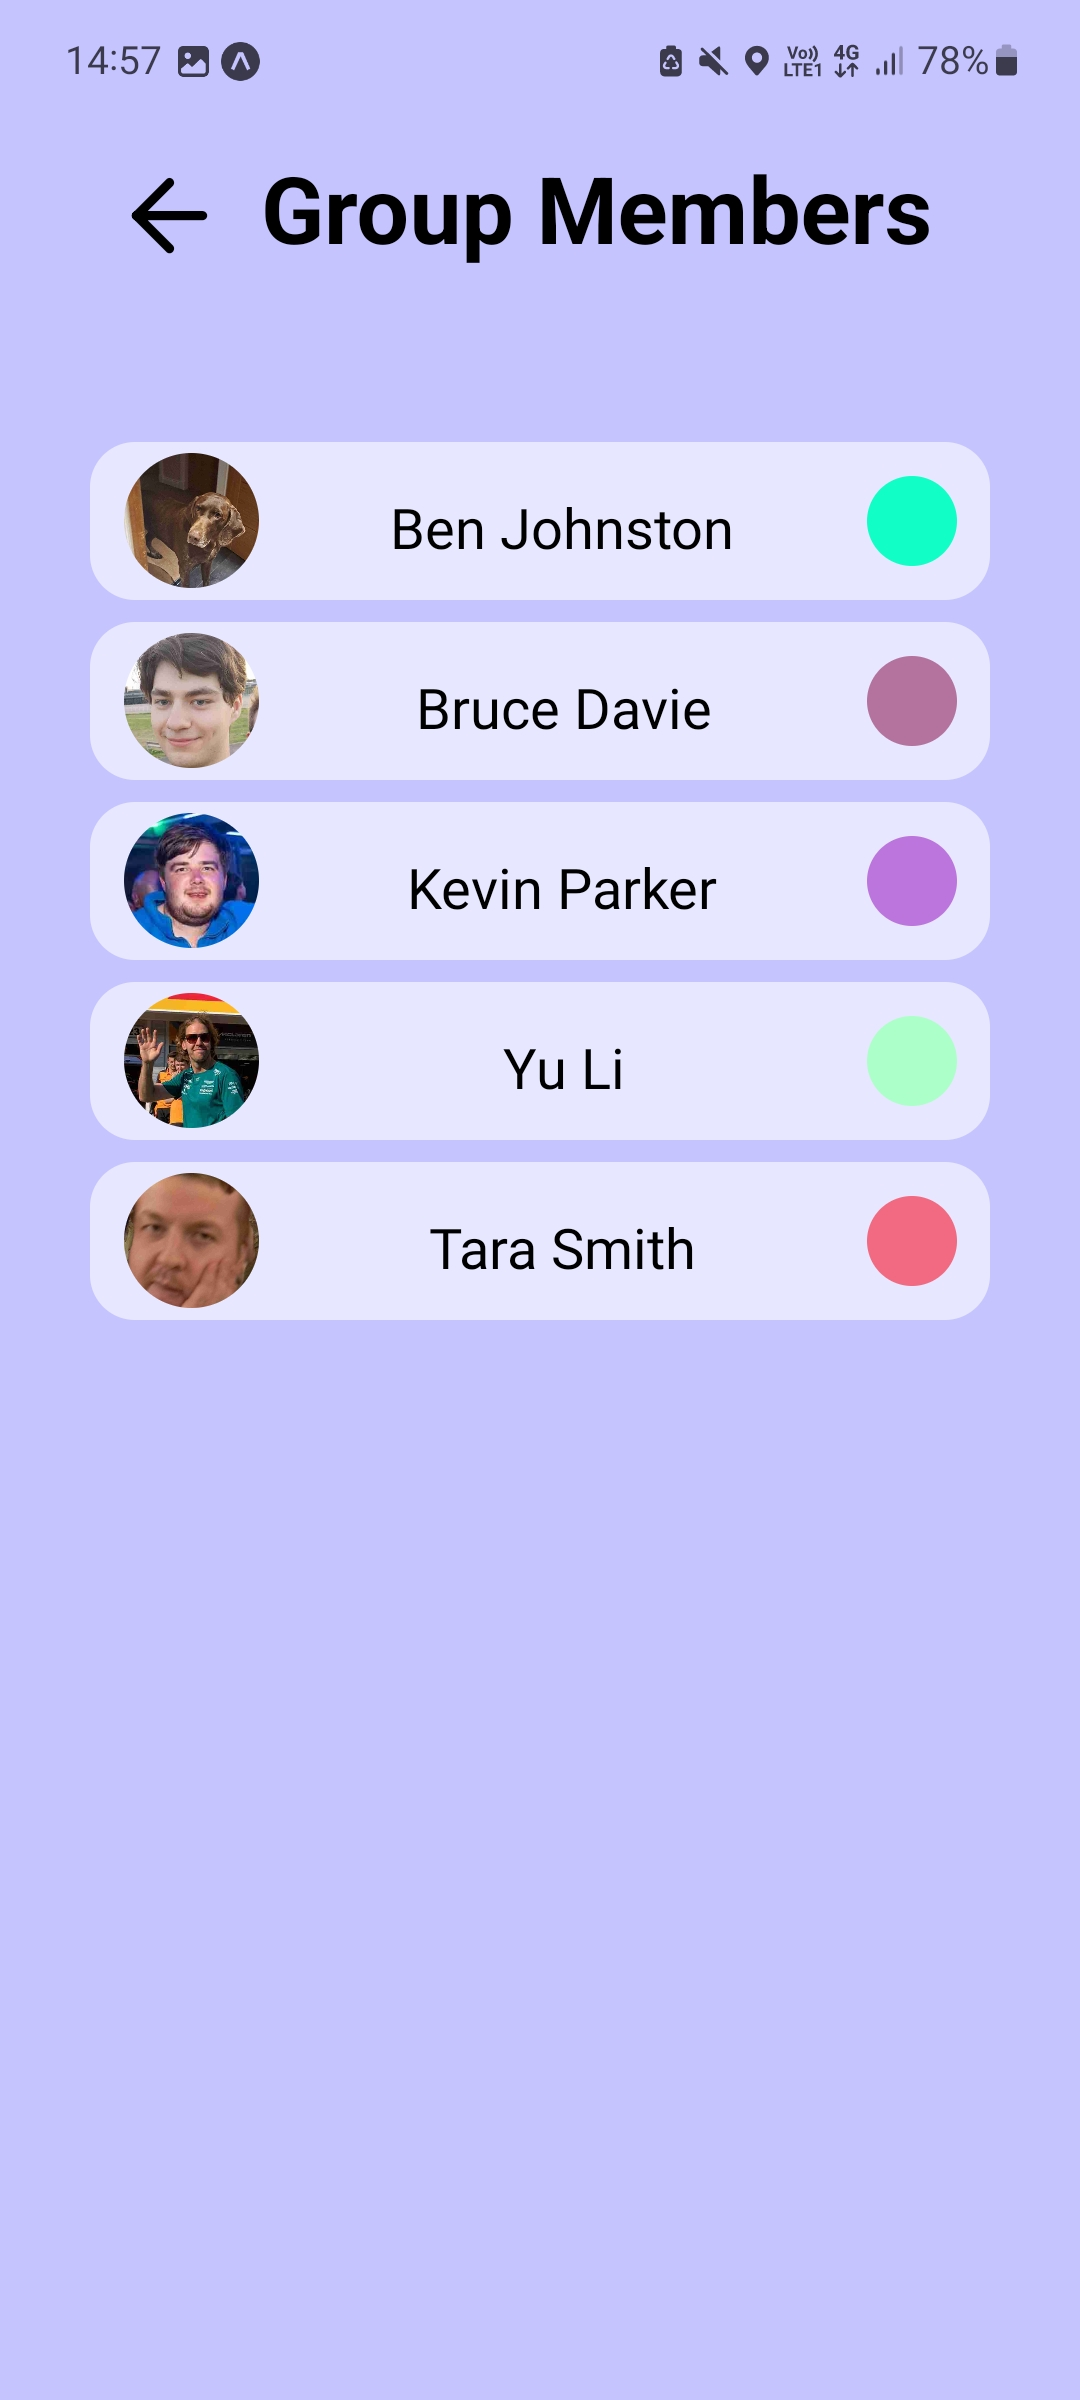
\includegraphics[width=\textwidth]{groupMembers.jpg}}
        \caption{Group Members}
    \end{subfigure}
    \vskip\baselineskip
    \noindent\begin{subfigure}[b]{0.23\textwidth}
        \centering
        \frame{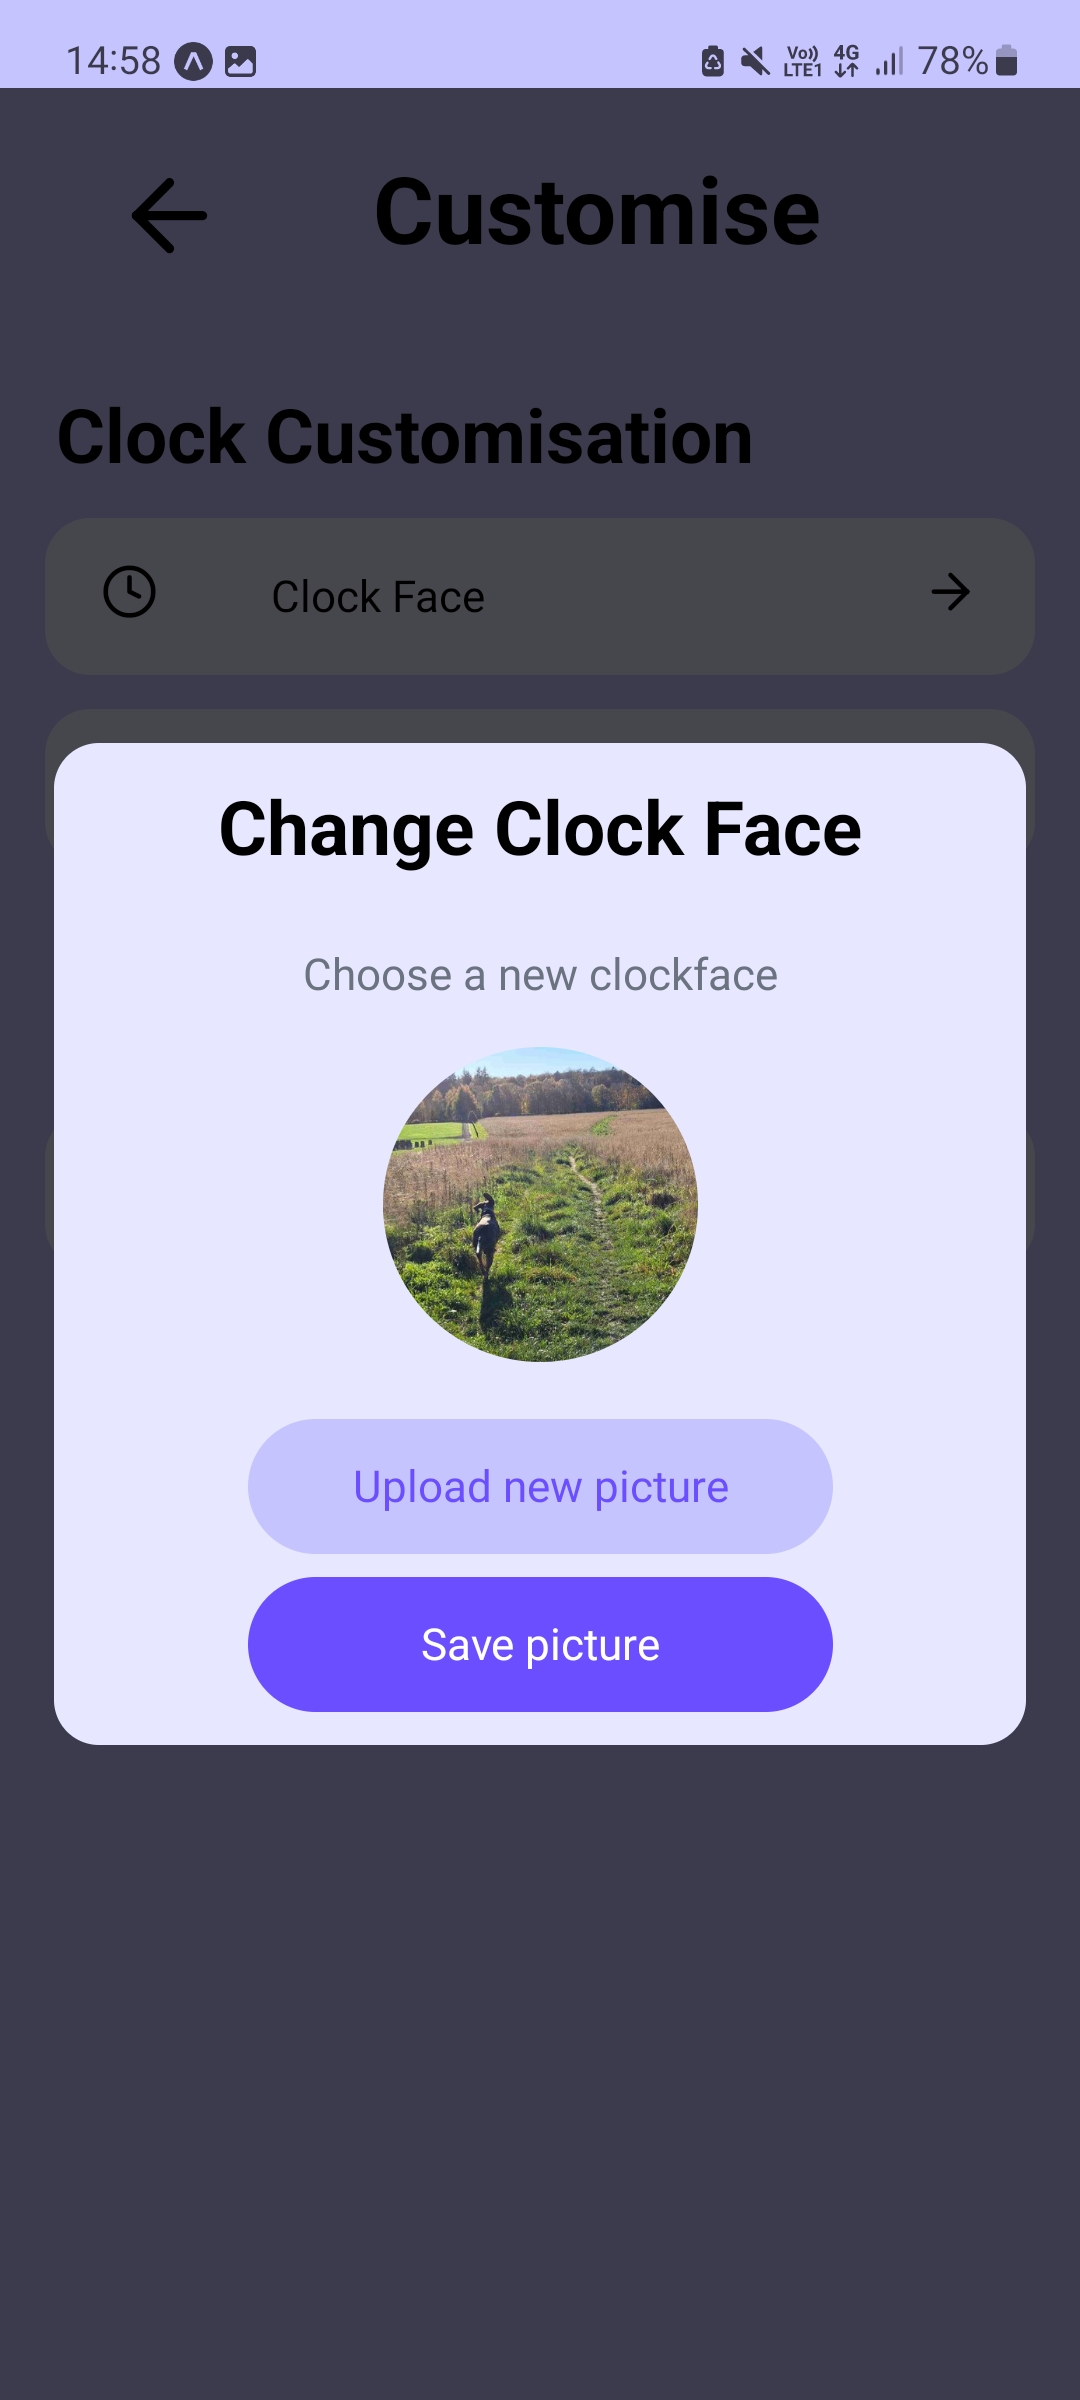
\includegraphics[width=\textwidth]{clockImg.jpg}}
        \caption{Clock Image Upload}
    \end{subfigure}
    \hspace{0.5em}
    \noindent\begin{subfigure}[b]{0.23\textwidth}
        \centering
        \frame{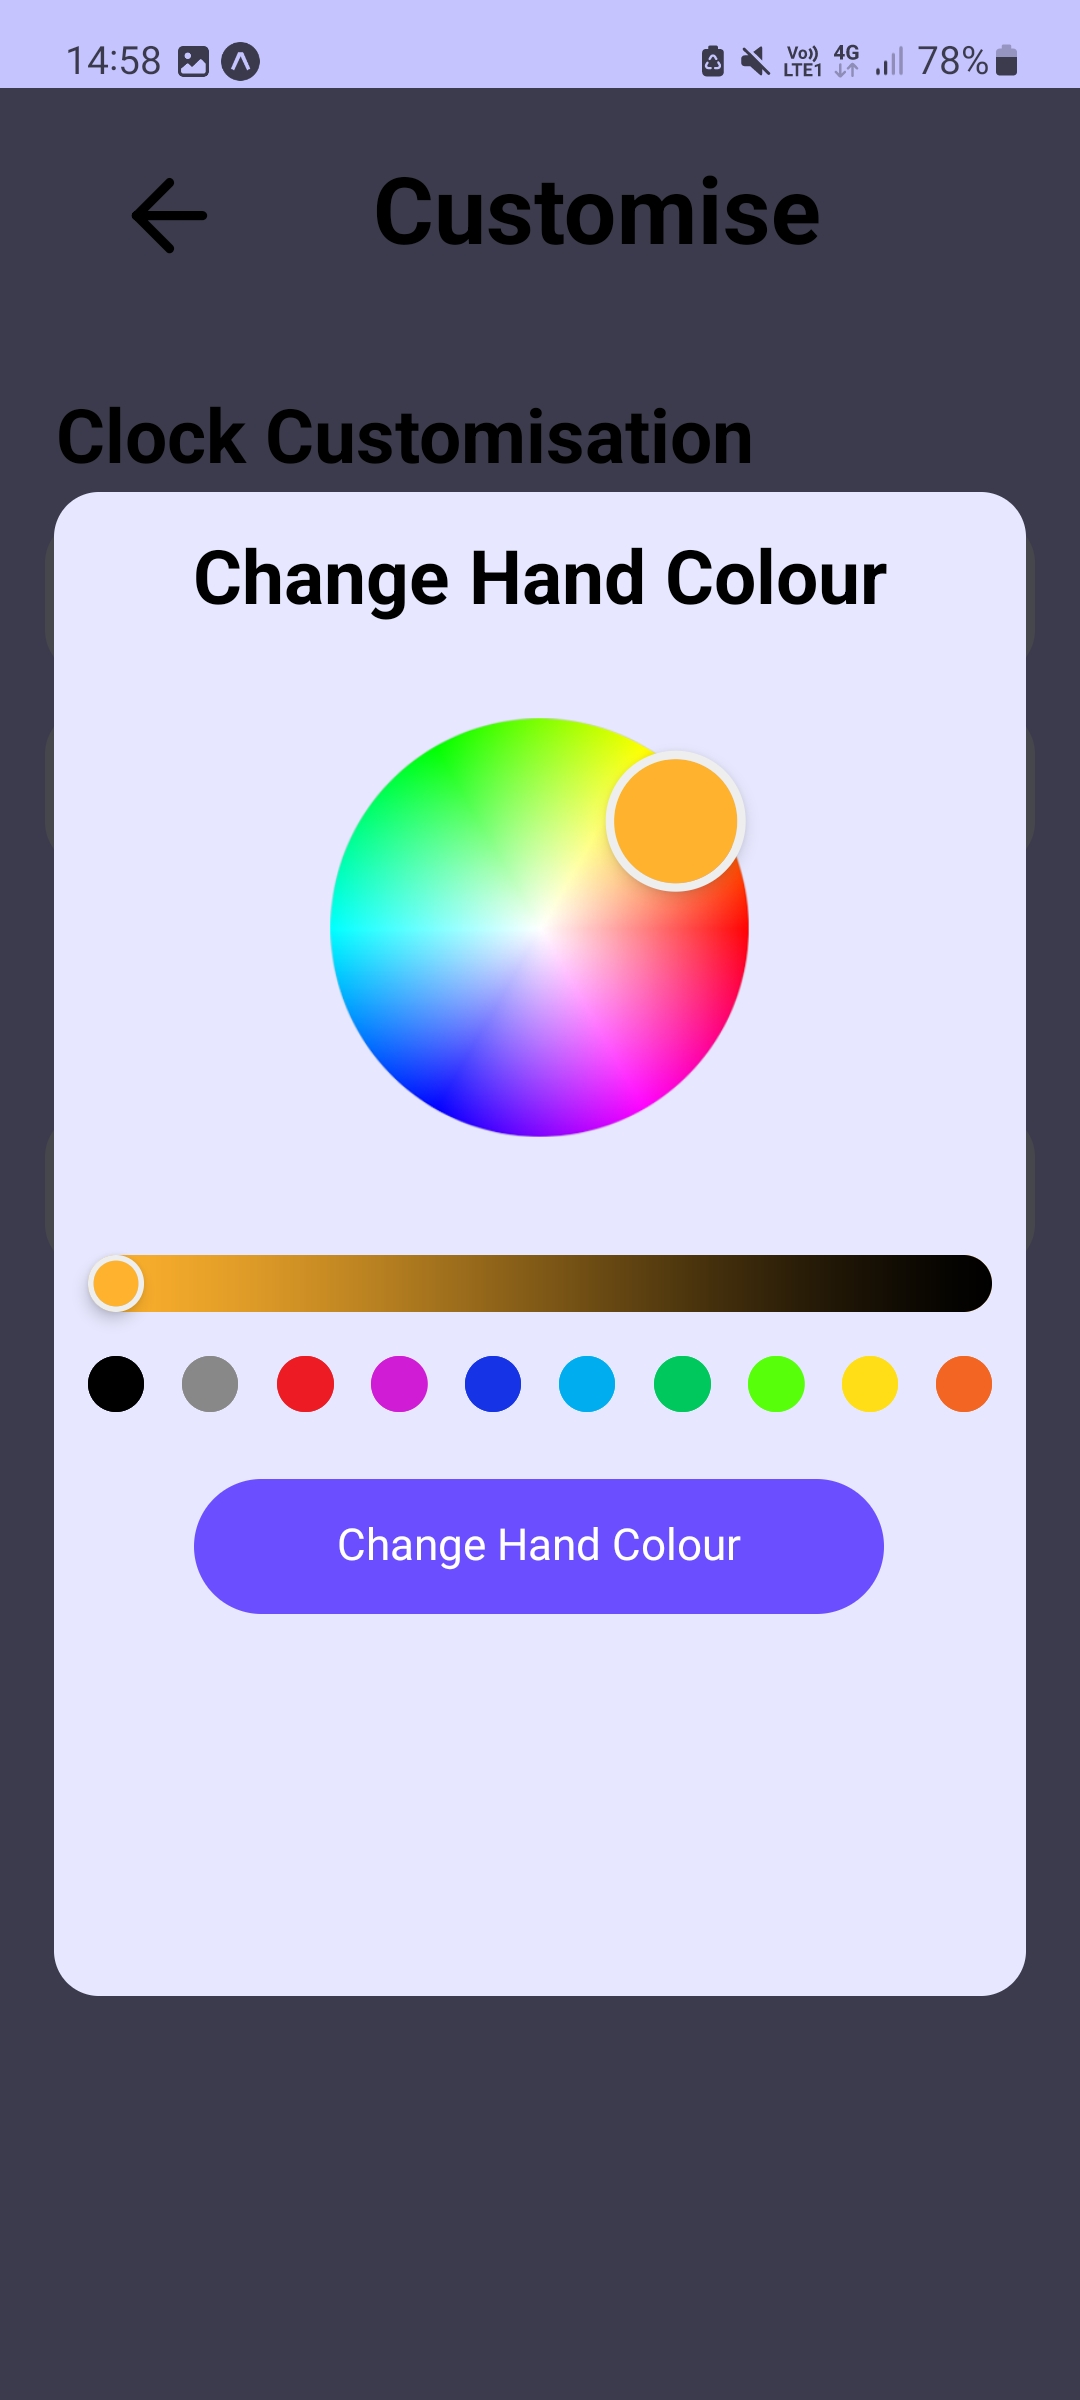
\includegraphics[width=\textwidth]{handCol.jpg}}
        \caption{Hand Colour Change}
    \end{subfigure}
    \hspace{0.5em}
    \noindent\begin{subfigure}[b]{0.23\textwidth}
        \centering
        \frame{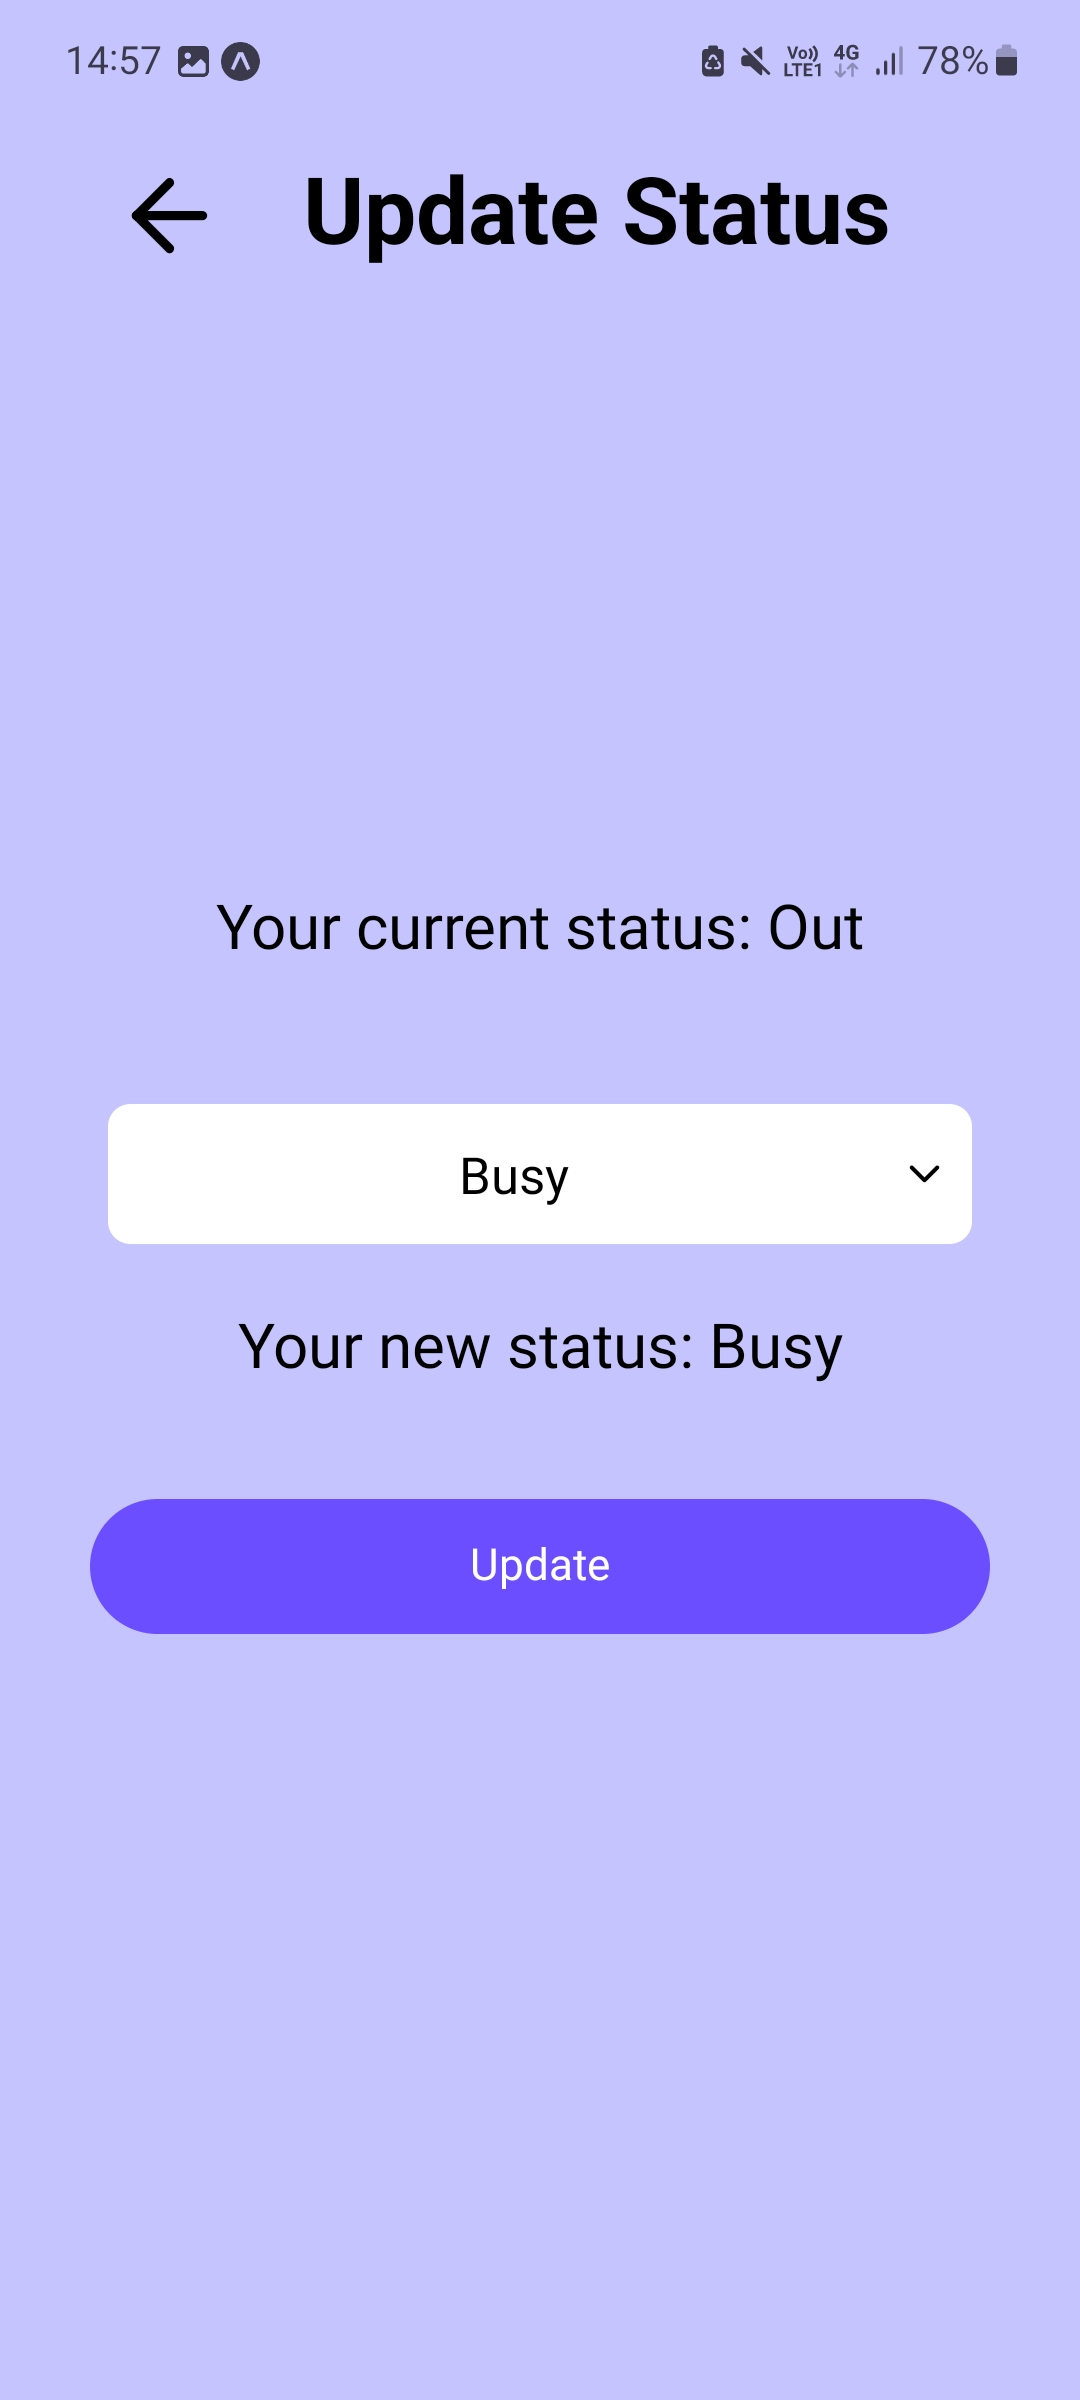
\includegraphics[width=\textwidth]{updateStat.jpg}}
        \caption{Update Status}
    \end{subfigure}
    \hspace{0.5em}
    \noindent\begin{subfigure}[b]{0.23\textwidth}
        \centering
        \frame{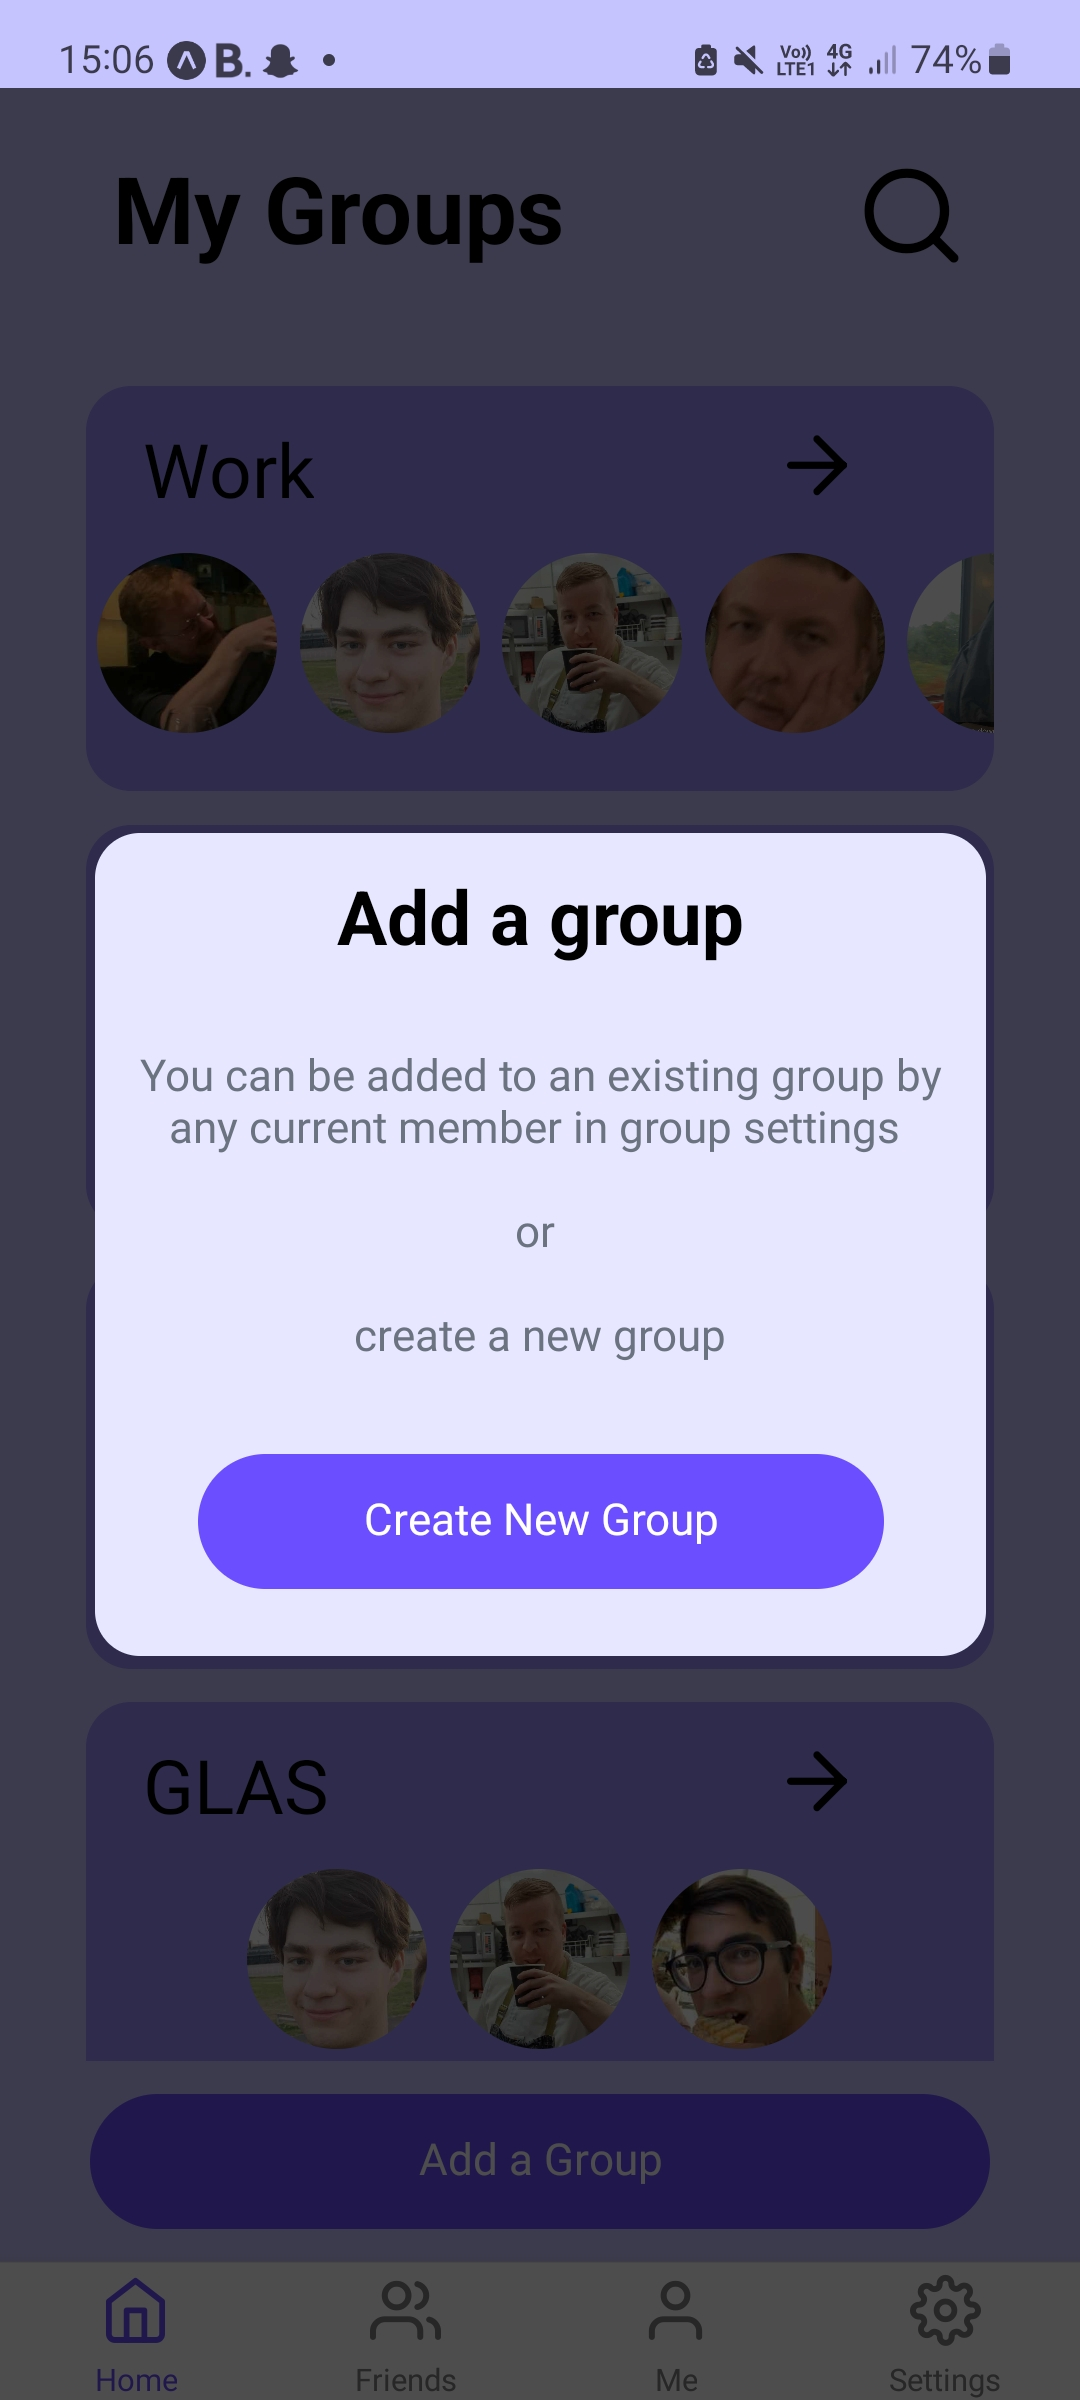
\includegraphics[width=\textwidth]{addGroup.jpg}}
        \caption{Add Group}
    \end{subfigure}
    \caption{Application pages}
\end{figure}
\FloatBarrier

\section{Reusable Component}\label{appendix:reusable}
\begin{figure}[!htbp]
    \centering
    \begin{subfigure}[b]{0.9\textwidth}
        \begin{lstlisting}[language=jsJsx]
        function AppButtonPurple(props) {
          const { title, onPressFunct } = props;
          return (
            <TouchableOpacity
              onPress={onPressFunct}
              className="bg-darkerPurple h-12 w-10/12 pt-3 rounded-full mx-1.5"
            >
              <Text className="text-white text-center">{title}</Text>
            </TouchableOpacity>
          );
        }
        
        AppButtonPurple.propTypes = {
          title: PropTypes.string.isRequired,
          onPressFunct: PropTypes.func.isRequired,
        };
        \end{lstlisting}
    \end{subfigure}
    \caption{Example of a reusable component}
    \small\textit{Here an onPress function and title are passed to this component to create a purple button with this title and onPress functionality. }
\end{figure}
\FloatBarrier

\section{Realtime database overview}\label{appendix:rtdb}
\begin{figure}[!htbp]
    \centering
    \begin{subfigure}[b]{\textwidth}
        \frame{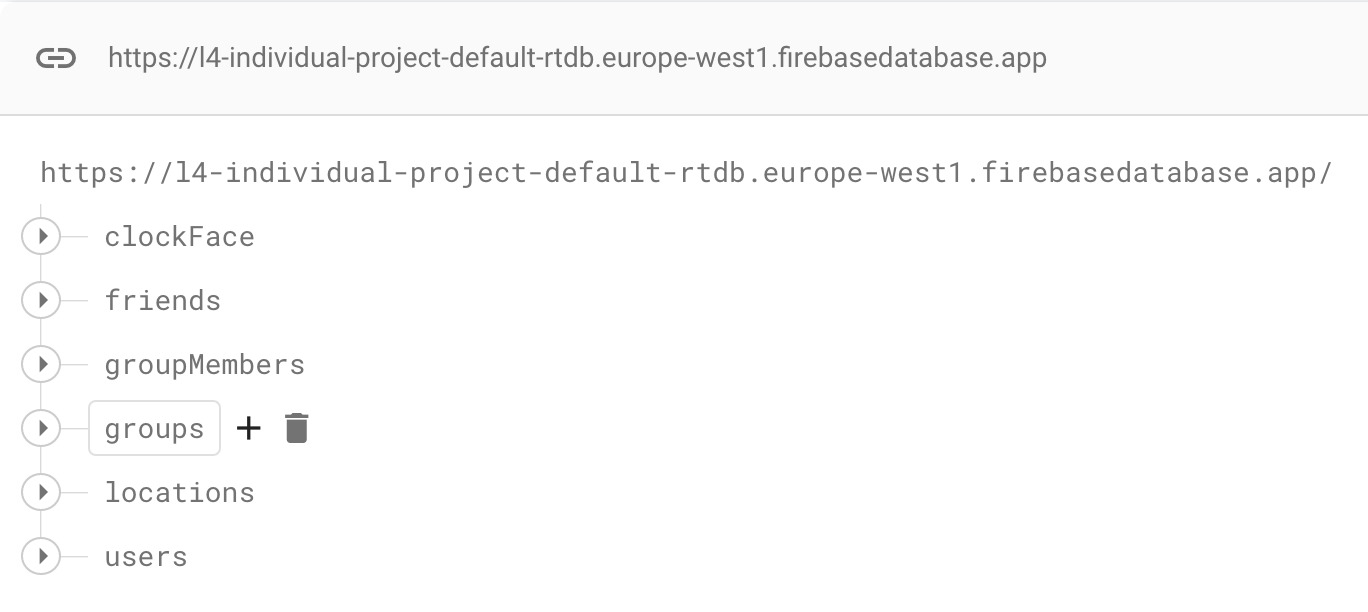
\includegraphics[width=\textwidth]{rtdb.png}}
    \end{subfigure}
    \caption{The JSON tree for the applications realtime database}
\end{figure}
\FloatBarrier
\newpage

\section{Realtime database security rules}\label{appendix:securityRulesRTDB}
\begin{figure}[!htbp]
    \centering
    \begin{subfigure}[b]{0.6\textwidth}
        \frame{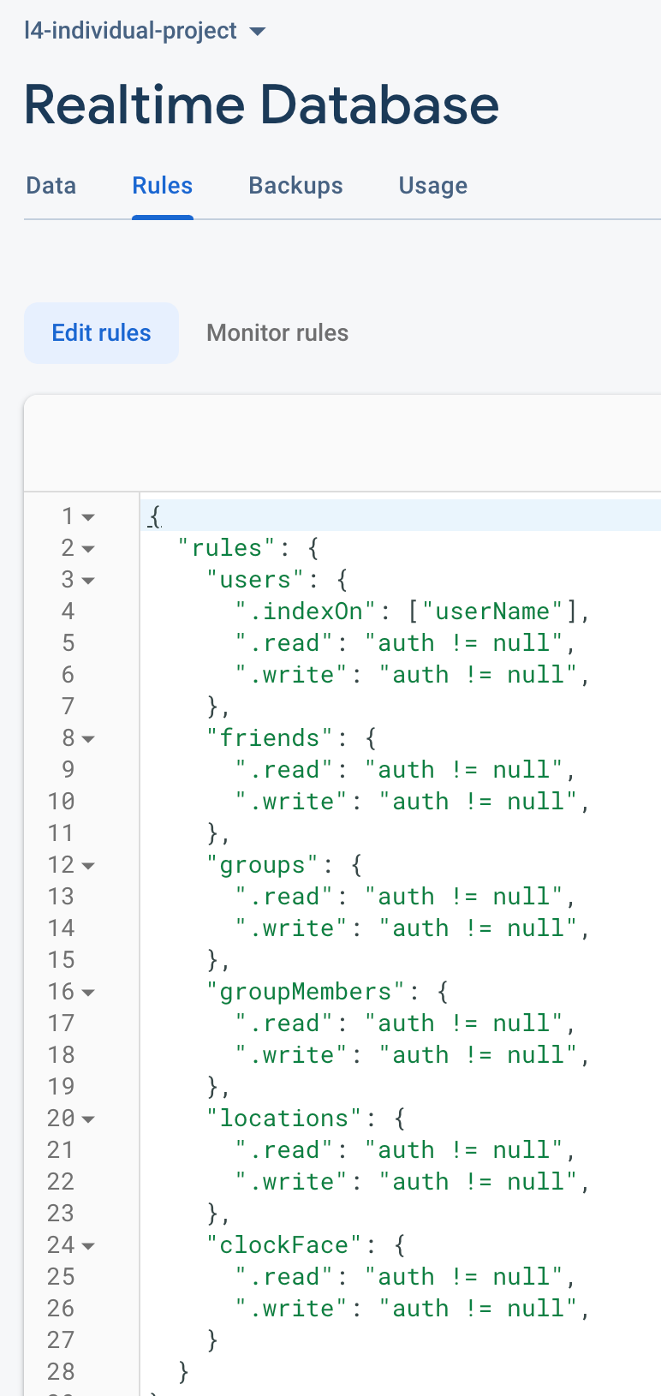
\includegraphics[width=\textwidth]{securityRulesRTDB.png}}
    \end{subfigure}
    \caption{The security rules for the realtime database}
    \small\textit{Here only an authenticated user can read, or, write to the database}
\end{figure}
\FloatBarrier
\newpage

\section{Storage security rules}\label{appendix:securityRulesStor}
\begin{figure}[!htbp]
    \centering
    \begin{subfigure}[b]{0.8\textwidth}
        \frame{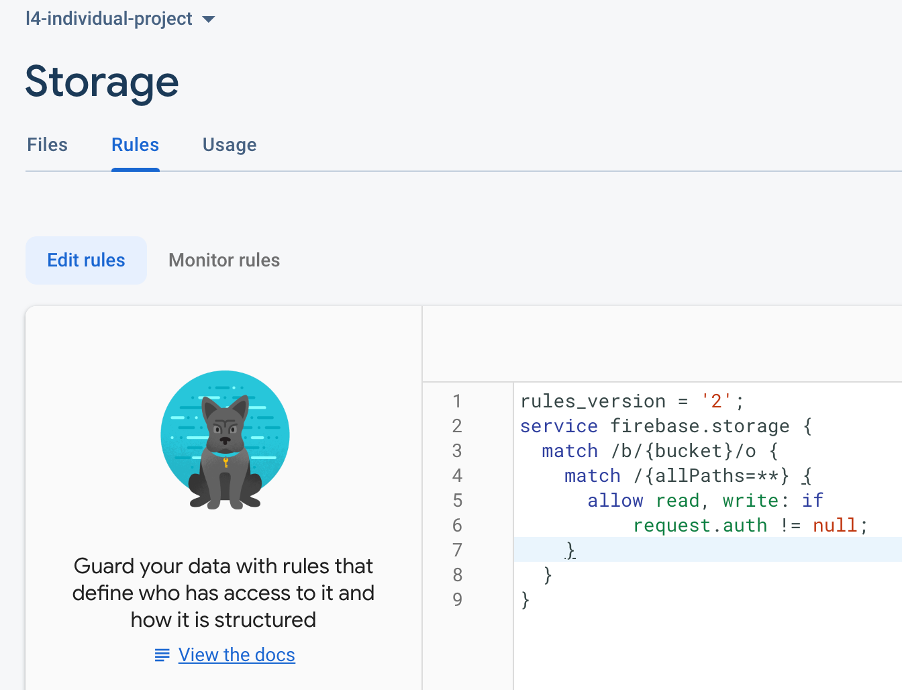
\includegraphics[width=\textwidth]{securityRulesStor.png}}
    \end{subfigure}
    \caption{The security rules for the cloud storage}
    \small\textit{Here only an authenticated user can read, or, write to the storage}
\end{figure}
\FloatBarrier

\section{Evaluation}
\subsection{Introductory Questions}\label{appendix:introQns}
\vskip\baselineskip
\begin{enumerate}
    \item Do you have issues with planning activities due to being unaware of your friend's status?
    \item Do you use snapchat maps or life360 for example to see what your friends are up to?
    \item Would you be likely to use an app to graphically see your friend's status?
\end{enumerate}
\vskip\baselineskip

\subsection{Tasks for in person evaluation}\label{appendix:tasks}
\vskip\baselineskip
\begin{enumerate}[label=Task \arabic*:]
    \item Please register for a new account and login
    \item Please logout and login with the credentials \newline
            Email - oz@gmail.com \newline
            Password - 12345678B \newline
        Now create a new group and add member `tdawg' \newline
        Now change the group name
    \item Please now change the clock-face to either a colour or an image, then change your hand colour
    \item Please now navigate to the friends screen and search for the user `wwall' and send them a friend request \newline
Now view your friends list and cancel this request
    \item Please now navigate to the your profile page and add a bio and a profile picture
\end{enumerate}
\vskip\baselineskip

\subsection{System Usability Scale Questions}\label{appendix:susQns}
\vskip\baselineskip
\begin{enumerate}
    \item I think that I would like to use this system frequently.
    \item I found the system unnecessarily complex.
    \item I thought the system was easy to use.
    \item I think that I would need the support of a technical person to be able to use this system.
    \item I found the various functions in this system were well integrated.
    \item I thought there was too much inconsistency in this system.
    \item I would imagine that most people would learn to use this system very quickly.
    \item I found the system very cumbersome to use.
    \item I felt very confident using the system.
    \item I needed to learn a lot of things before I could get going with this system.
\end{enumerate}
\vskip\baselineskip

\subsection{System Usability Scale Results}\label{appendix:susResults}
\begin{tabular}{ |c|c|c|c|c|c|c|c|c|c|c|c| } 

\hline
 \multicolumn{11}{|c|}{SUS Scores} \\
 \hline
 \hline
 Qn 1 & Qn 2 & Qn 3 & Qn 4 & Qn 5 & Qn 6 & Qn 7 & Qn 8 & Qn 9 & Qn 10 & SUS Score \\ [0.5ex] 
 \hline\hline
5 & 1 & 4 &	1 &	5 &	1 &	5 &	2 &	5 &	1 &	95 \\
 \hline
3 & 1 &	2 &	1 &	2 &	2 &	3 &	1 &	4 &	3 &	65 \\
 \hline
4 &	1 &	5 &	1 &	5 &	1 &	4 &	3 &	5 &	1 &	90 \\
 \hline
4 &	1 &	5 &	1 &	5 &	1 &	5 &	1 &	4 &	1 &	95 \\
 \hline
4 &	1 &	5 &	1 &	4 &	1 &	5 &	1 &	4 &	2 &	90 \\
 \hline
 3 &	1 &	4 &	1 &	4 &	1 &	5 &	4 &	5 &	5 &	72.5 \\
 \hline
 4 &	1 &	5 &	4 &	3 &	1 &	5 &	1 & 5 &	2 &	82.5 \\
 \hline
 4 &	2 &	4 &	1 &	4 &	2 &	5 &	1 &	4 &	1 &	85 \\
 \hline 
\end{tabular}

\begin{tabular}{ |c|c|c| } 
    \hline
     Average SUS Score & 84.38 & A+ \\ [0.5ex] 
     \hline

\end{tabular}

\subsection{Concluding Questions}\label{appendix:concludQns}
\vskip\baselineskip
\begin{enumerate}
    \item After using the app are you interested in the concept?
    \item Would you potentially use such an app?
    \item Are there any features you would change?
    \item Any extra feedback....
\end{enumerate}

\subsection{Online Evaluation Video Questions}\label{appendix:vidQns}
\vskip\baselineskip
\begin{enumerate}[label=Video \arabic*:]
    \item Register, Login, Editing of profile, Friends, Screen layout \newline
    Questions:
    \begin{enumerate}
        \item Did you think the app looked easy to navigate?
        \item Did you think the design of the screens was consistent?
        \item Do you think the level of customisation for profiles is sufficient?
        \item Any additional thoughts....
    \end{enumerate}
    \vskip\baselineskip
    \item Creation of a group, Group customisation, General groups operation\newline
    Questions:
    \begin{enumerate}
        \item Did you think this process looked easy to learn and perform?
        \item Did you think the design of the screens was consistent?
        \item Do you think the level of customisation for groups was sufficient?
        \item Any additional thoughts....
    \end{enumerate}

\end{enumerate}
\vskip\baselineskip

\subsection{Online Evaluation General Application Questions}\label{appendix:onlineGenQns}
\vskip\baselineskip
\begin{enumerate}
    \item I really liked the design of the application.
    \item I thought this app seemed very easy to use and navigate.
    \item I would imagine that most people would learn to use this system very quickly.
    \item I thought there was too much inconsistency in this system.
\end{enumerate}
\vskip\baselineskip

\subsection{Online Evaluation Question Responses}\label{appendix:onlineQnResp}
\vskip\baselineskip
All question responses are from a 1 - 5 scale, all questions except question 4 in general followed 1 as being the positive end of the scale, and, 5 as negative. For question 4 this is reversed.

\begin{table}[!ht]
    \centering
    \begin{tabular}{|l|l|l||l|l|l||l|l|l|l|}
    \hline
     \multicolumn{3}{|c||}{Video 1 } &
     \multicolumn{3}{|c||}{Video 2 } &
     \multicolumn{4}{|c|}{General } \\
    \hline
        \textbf{a} & \textbf{b} & \textbf{c} & \textbf{a} & \textbf{b} & \textbf{c} & \textbf{1} & \textbf{2} & \textbf{3} & \textbf{4} \\ \hline\hline
        1 & 1 & 1 & 1 & 1 & 2 & 2 & 1 & 1 & 4 \\ \hline
        1 & 1 & 2 & 2 & 1 & 1 & 1 & 1 & 2 & 5 \\ \hline
        1 & 1 & 1 & 1 & 1 & 1 & 1 & 1 & 2 & 4 \\ \hline
        1 & 1 & 2 & 2 & 1 & 1 & 2 & 2 & 1 & 5 \\ \hline
        1 & 1 & 1 & 1 & 1 & 1 & 1 & 1 & 1 & 5 \\ \hline
        1 & 1 & 1 & 1 & 1 & 1 & 2 & 1 & 1 & 5 \\ \hline
        1 & 1 & 1 & 1 & 1 & 1 & 1 & 1 & 1 & 5 \\ \hline
        2 & 1 & 1 & 2 & 1 & 1 & 4 & 2 & 2 & 4 \\ \hline
        2 & 1 & 2 & 1 & 1 & 3 & 2 & 1 & 1 & 5 \\ \hline
        2 & 1 & 1 & 1 & 1 & 1 & 1 & 1 & 1 & 4 \\ \hline
        2 & 1 & 2 & 1 & 1 & 2 & 2 & 1 & 1 & 5 \\ \hline
        2 & 1 & 2 & 3 & 1 & 1 & 2 & 1 & 1 & 5 \\ \hline
        2 & 5 & 2 & 1 & 2 & 1 & 1 & 2 & 2 & 5 \\ \hline
        2 & 1 & 2 & 3 & 2 & 2 & 2 & 2 & 1 & 4 \\ \hline
        2 & 1 & 2 & 2 & 2 & 1 & 2 & 4 & 2 & 4 \\ \hline
        3 & 2 & 2 & 2 & 1 & 2 & 2 & 2 & 1 & 4 \\ \hline
        1 & 2 & 2 & 1 & 2 & 1 & 2 & 1 & 1 & 4 \\ \hline
        1 & 1 & 1 & 1 & 1 & 1 & 1 & 1 & 1 & 5 \\ \hline
        1 & 1 & 1 & 2 & 1 & 2 & 2 & 2 & 1 & 5 \\ \hline
        1 & 1 & 1 & 1 & 1 & 1 & 1 & 1 & 1 & 5 \\ \hline
        1 & 1 & 1 & 1 & 1 & 1 & 1 & 1 & 1 & 5 \\ \hline
        2 & 1 & 2 & 1 & 2 & 2 & 2 & 1 & 1 & 4 \\ \hline
        2 & 1 & 1 & 1 & 1 & 1 & 2 & 2 & 2 & 5 \\ \hline
        1 & 2 & 2 & 1 & 1 & 1 & 3 & 1 & 1 & 4 \\ \hline
    \end{tabular}
\end{table}


\addtocontents{toc}{\setcounter{tocdepth}{1}}